\chapter{Proteins as machines}
\label{vol06:ch04}

\epigraph{The native conformation is determined by the totality of
interatomic interactions and hence by the amino acid sequence, in a
given environment.}{Christian B. Anfinsen, Nobel lecture (1972), in
\emph{Science} 181:223--230 \cite[p.~223]{paper:anfinsen1973-protein-folding}.}

\chapmeta{Half-life: foundational. Archetypes: control, scaling. Exercise target: 25. Project track: visualisation and structure-function analysis of three proteins from the Protein Data Bank using free molecular-viewer software. Hazard class: none (computational work only). Reader path default: standard, with sections explicitly tagged. Named cases: none required; misfolding diseases (Alzheimer's, prion diseases, sickle cell) are described as mechanism classes rather than named registry events.}

\noindent
Proteins are the cell's machines. Each protein is a polypeptide chain
that has folded into a specific three-dimensional shape, and the
shape is what makes the protein do what it does. The chapter develops
the protein-as-machine reading of cellular biology: it walks from the
amino-acid primary structure through the folding process to the
functional classes (enzymes, motors, channels, pumps), introduces
allosteric regulation as the cell's principal mechanism for tuning
enzymatic activity, and closes with the failure modes that arise when
proteins fold incorrectly or fail to maintain their structure under
load.

\section{Amino acids and primary structure}\pathtag{core}

A \engterm{protein} is a linear polymer of amino acids joined by
peptide bonds. The cell uses $20$ standard amino acids, plus the two
non-standard amino acids selenocysteine and pyrrolysine that some
organisms encode through specific recoding mechanisms. Each amino
acid has the same backbone (an amino group, a central $\alpha$-carbon,
and a carboxylic acid group) and a distinct side chain. The $20$
side chains span a chemical range that includes hydrophobic
(alanine, valine, leucine, isoleucine, methionine, phenylalanine,
tryptophan), polar uncharged (serine, threonine, asparagine,
glutamine, tyrosine), charged (aspartate and glutamate negative,
lysine and arginine positive, histidine positive at physiological pH
of $7.4$ with $\text{pK}_a \approx 6.0$), special (glycine with no
side chain, proline with a cyclic side chain, cysteine with a thiol
that can form disulfide bonds) \cite[ch.~3]{text:lehninger-biochemistry}.
The chemical inventory is tabulated, with side-chain properties and
amino-acid frequencies in the Swiss-Prot 2024 release, in the chapter's
\path{data/amino_acid_properties.csv} dataset and visualised in
Figure~\ref{fig:v6c04-aa-classes}.

\begin{figure}[ht]
\centering
% Amino-acid R-group classification panel.
% Boxes for each of the twenty amino acids, grouped by chemical class.
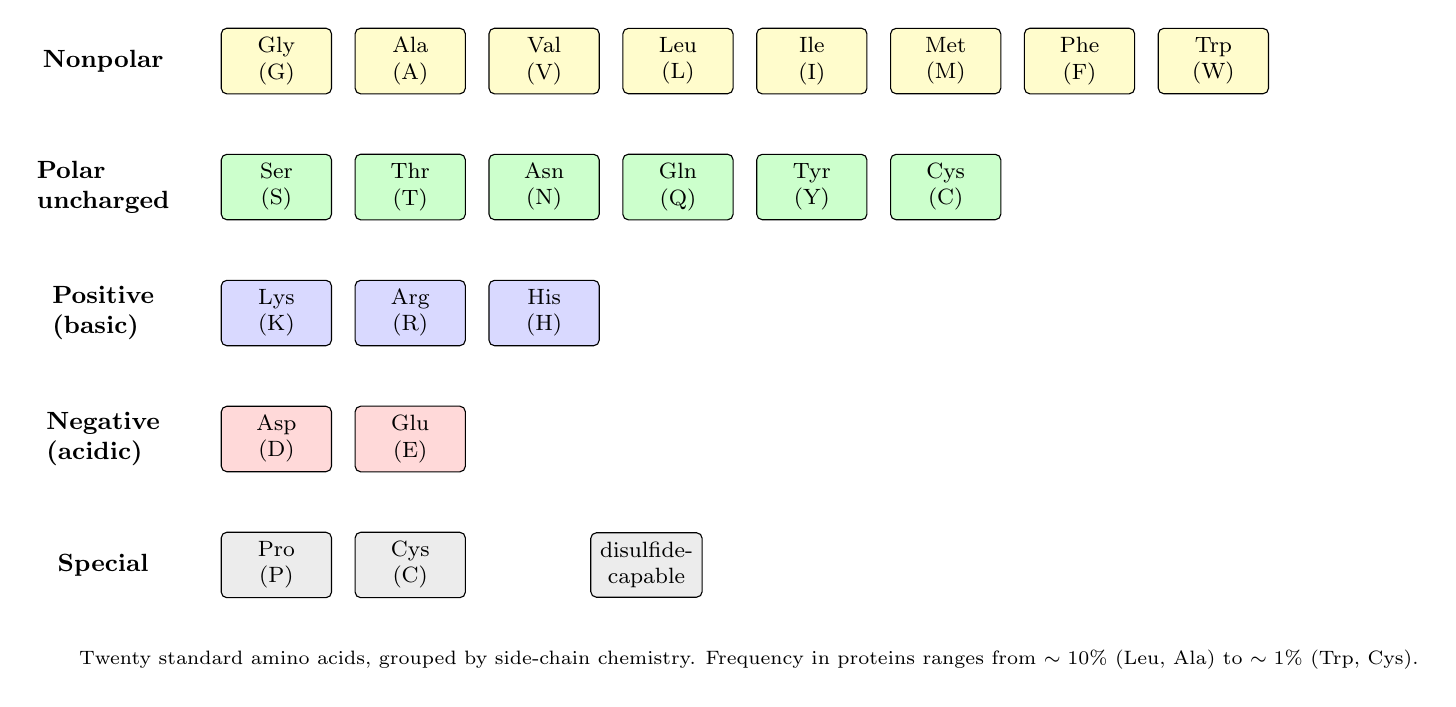
\begin{tikzpicture}[
    aa/.style={draw, rounded corners=2pt, minimum width=1.4cm,
               minimum height=0.8cm, font=\footnotesize, align=center},
    nonpolar/.style={aa, fill=yellow!20},
    polar/.style={aa, fill=green!20},
    positive/.style={aa, fill=blue!15},
    negative/.style={aa, fill=red!15},
    special/.style={aa, fill=gray!15},
    class/.style={font=\small\bfseries, align=left},
]
\node[class] at (-1.2, 5.6) {Nonpolar};
\node[nonpolar] at (1.0, 5.6) {Gly\\(G)};
\node[nonpolar] at (2.7, 5.6) {Ala\\(A)};
\node[nonpolar] at (4.4, 5.6) {Val\\(V)};
\node[nonpolar] at (6.1, 5.6) {Leu\\(L)};
\node[nonpolar] at (7.8, 5.6) {Ile\\(I)};
\node[nonpolar] at (9.5, 5.6) {Met\\(M)};
\node[nonpolar] at (11.2, 5.6) {Phe\\(F)};
\node[nonpolar] at (12.9, 5.6) {Trp\\(W)};

\node[class] at (-1.2, 4.0) {Polar\\uncharged};
\node[polar] at (1.0, 4.0) {Ser\\(S)};
\node[polar] at (2.7, 4.0) {Thr\\(T)};
\node[polar] at (4.4, 4.0) {Asn\\(N)};
\node[polar] at (6.1, 4.0) {Gln\\(Q)};
\node[polar] at (7.8, 4.0) {Tyr\\(Y)};
\node[polar] at (9.5, 4.0) {Cys\\(C)};

\node[class] at (-1.2, 2.4) {Positive\\(basic)};
\node[positive] at (1.0, 2.4) {Lys\\(K)};
\node[positive] at (2.7, 2.4) {Arg\\(R)};
\node[positive] at (4.4, 2.4) {His\\(H)};

\node[class] at (-1.2, 0.8) {Negative\\(acidic)};
\node[negative] at (1.0, 0.8) {Asp\\(D)};
\node[negative] at (2.7, 0.8) {Glu\\(E)};

\node[class] at (-1.2, -0.8) {Special};
\node[special] at (1.0, -0.8) {Pro\\(P)};
\node[special] at (2.7, -0.8) {Cys\\(C)};
\node[special, font=\footnotesize] at (5.7, -0.8) {disulfide-\\capable};

\node[align=left, font=\scriptsize, anchor=west] at (5.5, -0.8) {};

\node[align=center, font=\scriptsize] at (7.0, -2.0)
    {Twenty standard amino acids, grouped by side-chain chemistry.
     Frequency in proteins ranges from $\sim 10\%$ (Leu, Ala) to $\sim 1\%$ (Trp, Cys).};
\end{tikzpicture}

\caption{The twenty standard amino acids, grouped by side-chain
chemistry. The colour coding distinguishes hydrophobic, polar uncharged,
positively charged, negatively charged, and special residues (glycine,
proline, cysteine). Leucine, alanine, glycine, and valine each
account for $\sim 7$ to $10\%$ of residues in the average protein;
tryptophan, cysteine, and histidine each account for $\sim 1$ to
$2\%$.}
\label{fig:v6c04-aa-classes}
\end{figure}

\engterm{The peptide bond}. The peptide bond is an amide bond between
the carboxyl carbon of one amino acid and the amino nitrogen of the
next. The bond has partial double-bond character (delocalised
resonance with the adjacent carbonyl), which makes it planar and
restricts the polypeptide backbone to two rotational degrees of
freedom per residue: the $\phi$ angle (rotation around the
$\text{N}-\text{C}_\alpha$ bond) and the $\psi$ angle (rotation around
the $\text{C}_\alpha-\text{C}$ bond). The allowed combinations of
$\phi$ and $\psi$ form the \engterm{Ramachandran plot}
\cite{paper:v6c04-ramachandran-1963}, with three principal regions
corresponding to right-handed $\alpha$-helix
($\phi \approx -60^{\circ}$, $\psi \approx -45^{\circ}$),
$\beta$-sheet ($\phi \approx -135^{\circ}$, $\psi \approx +135^{\circ}$),
and left-handed $\alpha$-helix (rare, found in glycine-rich loops).
The plot's empty regions correspond to side-chain steric clashes
that no amino acid can fit. The Ramachandran plot is the working
diagnostic for whether a proposed protein structure is sterically
plausible.

\engterm{Primary, secondary, tertiary, quaternary structure}. Protein
structure is described at four hierarchical levels. \engterm{Primary
structure} is the amino-acid sequence. \engterm{Secondary structure}
is the local arrangement of the backbone into regular elements: the
$\alpha$-helix (a right-handed coil with $3.6$ residues per turn,
$0.54\,\text{nm}$ rise per turn, hydrogen bonds between the carbonyl
of residue $i$ and the amide of residue $i+4$), and the
$\beta$-sheet (parallel or antiparallel strands hydrogen-bonded
side-by-side, $0.7\,\text{nm}$ per residue along the strand). Both
secondary-structure elements were predicted by Linus Pauling and
Robert Corey in 1951 from model-building constraints, before any
high-resolution protein structure was available
\cite{paper:v6c04-pauling-corey-1951}; the predictions were confirmed
by the first X-ray crystal structures of myoglobin and haemoglobin in
1958 to 1960. \engterm{Tertiary structure} is the overall
three-dimensional fold of the polypeptide chain. \engterm{Quaternary
structure} is the assembly of multiple polypeptide chains into a
functional complex (haemoglobin, two $\alpha$ and two $\beta$ chains;
the proteasome, $28$ subunits; the ribosome, $\sim 80$ proteins plus
several RNAs). Figure~\ref{fig:v6c04-secondary} sketches the geometry
of the two principal secondary-structure elements.

\begin{figure}[ht]
\centering
% Alpha-helix and beta-sheet secondary structures with hydrogen-bond geometry.
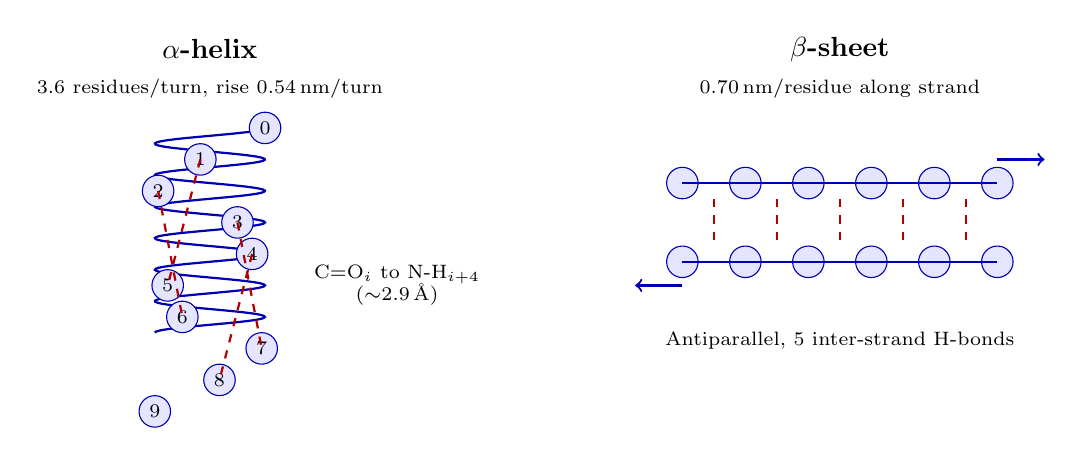
\begin{tikzpicture}[
    backbone/.style={thick, blue!70!black},
    hbond/.style={dashed, red!70!black, thick},
    res/.style={circle, draw=blue!70!black, fill=blue!10, inner sep=1pt,
                minimum size=4mm, font=\scriptsize},
    label/.style={font=\scriptsize, align=center},
]

% Left panel: alpha-helix backbone schematic
\begin{scope}[shift={(0,0)}]
\node[font=\bfseries] at (2.0, 4.5) {$\alpha$-helix};
\node[label] at (2.0, 4.0) {3.6 residues/turn, rise 0.54\,nm/turn};

% Helical path
\draw[backbone, domain=0:6.5, samples=200, smooth, variable=\t]
    plot ({2.0 + 0.7*cos(360*\t)}, {3.5 - 0.4*\t});

% Residue dots
\foreach \i in {0,...,9}{
  \node[res] at ({2.0 + 0.7*cos(360*\i/3.6)}, {3.5 - 0.4*\i}) {\i};
}

% Hydrogen bonds: residue i to i+4
\foreach \i/\j in {1/5, 2/6, 3/7, 4/8}{
  \draw[hbond] ({2.0 + 0.7*cos(360*\i/3.6)}, {3.5 - 0.4*\i})
       -- ({2.0 + 0.7*cos(360*\j/3.6)}, {3.5 - 0.4*\j});
}
\node[label, anchor=west] at (3.2, 1.5) {C=O$_i$ to N-H$_{i+4}$\\($\sim$2.9\,\AA)};
\end{scope}

% Right panel: antiparallel beta-sheet
\begin{scope}[shift={(7,0)}]
\node[font=\bfseries] at (3.0, 4.5) {$\beta$-sheet};
\node[label] at (3.0, 4.0) {0.70\,nm/residue along strand};

% Strand 1: residues 1-6 going right
\foreach \i in {0,...,5}{
  \node[res] at ({1.0 + 0.8*\i}, 2.8) {};
}
\draw[backbone] (1.0,2.8) -- (5.0,2.8);

% Strand 2: residues 7-12 going left
\foreach \i in {0,...,5}{
  \node[res] at ({1.0 + 0.8*\i}, 1.8) {};
}
\draw[backbone] (1.0,1.8) -- (5.0,1.8);

% H-bonds between strands
\foreach \x in {1.4, 2.2, 3.0, 3.8, 4.6}{
  \draw[hbond] (\x, 2.6) -- (\x, 2.0);
}

\draw[->, thick, blue!70!black] (5.0, 3.1) -- (5.6, 3.1);
\draw[->, thick, blue!70!black] (1.0, 1.5) -- (0.4, 1.5);
\node[label] at (3.0, 0.8) {Antiparallel, 5 inter-strand H-bonds};
\end{scope}

\end{tikzpicture}

\caption{Secondary structure. Left: a right-handed $\alpha$-helix with
$3.6$ residues per turn and $0.54\,\text{nm}$ rise per turn; hydrogen
bonds (dashed) connect the carbonyl of residue $i$ to the amide of
residue $i+4$ at an $\text{O} \cdots \text{N}$ distance of
approximately $2.9\,\si{\angstrom}$. Right: an antiparallel
$\beta$-sheet with inter-strand hydrogen bonds and a strand-direction
arrow.}
\label{fig:v6c04-secondary}
\end{figure}

\engterm{Bond budget}. The free energy of a folded protein is the sum
of contributions from: hydrogen bonds within the backbone (typically
$10$ to $30\,\text{kJ}/\text{mol}$ per hydrogen bond, although
buried hydrogen bonds in the protein interior can be stronger);
hydrophobic burial of non-polar side chains (the dominant driving
force for folding, accounting for $50$ to $100\,\text{kJ}/\text{mol}$
of stability for a typical small protein); electrostatic interactions
between charged side chains ($5$ to $20\,\text{kJ}/\text{mol}$ for
buried salt bridges); van der Waals packing in the protein core; and
disulfide bonds in extracellular proteins ($\sim 100\,\text{kJ}/\text{mol}$
each, but only present in oxidising environments). The net stability
of a typical folded protein over its unfolded reference state is
$20$ to $60\,\text{kJ}/\text{mol}$, a small number that is the
difference of two large contributions (favourable enthalpic and
hydrophobic interactions, unfavourable entropy of folding). The
small net stability is the engineering reading of protein
\engterm{marginal stability}: most proteins are just stable enough
to maintain their fold under physiological conditions, and modest
perturbations (temperature, pH, denaturants) can unfold them
\cite[ch.~4]{text:branden-tooze-proteins,text:v6c04-creighton-proteins-1993}.

\engterm{Worked example: $\alpha$-helix geometry}. The $\alpha$-helix
parameters yield a few useful consequences. With $3.6$ residues per
turn and $0.54\,\text{nm}$ rise per turn, the rise per residue is
$h = 0.54/3.6 = 0.150\,\text{nm}$. A typical $\alpha$-helical segment
of a globular protein has $10$ to $20$ residues, giving a length of
$1.5$ to $3.0\,\text{nm}$. A transmembrane helix that spans a
$\sim 3\,\text{nm}$ hydrophobic bilayer core needs $3.0/0.15 = 20$
residues; this is the textbook membrane-protein helix length and the
basis of hydropathy-plot prediction of membrane topology. The pitch
per turn ($0.54\,\text{nm}$) sets the apparent stripe spacing in
cryo-electron tomograms of helical regions and the
$\sim 5.4\,\si{\angstrom}$ meridional reflection in fibre diffraction.

\section{Protein folding}\pathtag{standard}

A protein's three-dimensional structure is, in most cases,
determined by its amino-acid sequence under the cell's solvent and
temperature conditions. The thermodynamic hypothesis, due to Christian
Anfinsen's 1962 ribonuclease refolding experiments, states that the
native conformation is the global free-energy minimum of the
polypeptide in its physiological environment
\cite{paper:anfinsen1973-protein-folding,paper:v6c04-anfinsen-1973}.
The hypothesis has been confirmed for most small, single-domain
proteins by their ability to refold spontaneously after chemical
denaturation; for larger or more complex proteins, the folding is
kinetically assisted by \engterm{chaperone} proteins that prevent
off-pathway aggregation but do not alter the final structure
\cite{paper:v6c04-saibil-chaperones-2013}.

\engterm{Levinthal's paradox and the folding funnel}. A protein of
$N$ residues with three rotational states per residue would have
$3^N$ possible conformations; for $N = 100$, the number is $5 \times
10^{47}$ \cite{paper:v6c04-levinthal-1968}. If folding proceeded by
random search through all conformations at the fastest single-bond
rotation timescale ($\sim 1\,\text{ps}$), the time required would be
$5 \times 10^{35}\,\text{s}$, twenty-eight orders of magnitude longer
than the age of the universe. Proteins, however, fold in microseconds
to seconds. The resolution, due to Wolynes, Bryngelson, and others in
the 1980s and 1990s, is that the folding-energy landscape is not
flat but has a \engterm{folding funnel} shape: the native state is
at the bottom of a broad, downhill-biased energy landscape that
channels the polypeptide toward the native state regardless of the
starting conformation \cite{paper:v6c04-bryngelson-wolynes-1987}. The
funnel shape is itself a result of evolutionary selection: protein
sequences that fold reliably are the ones that survived. The
folding-funnel framing is the modern engineering reading of protein
folding and the basis of most computational structure-prediction
methods \cite[ch.~6]{text:dill-bromberg-molecular-driving}.
Figure~\ref{fig:v6c04-funnel} sketches the funnel diagram with three
illustrative trajectories.

\begin{figure}[ht]
\centering
% Protein folding energy landscape (funnel diagram).
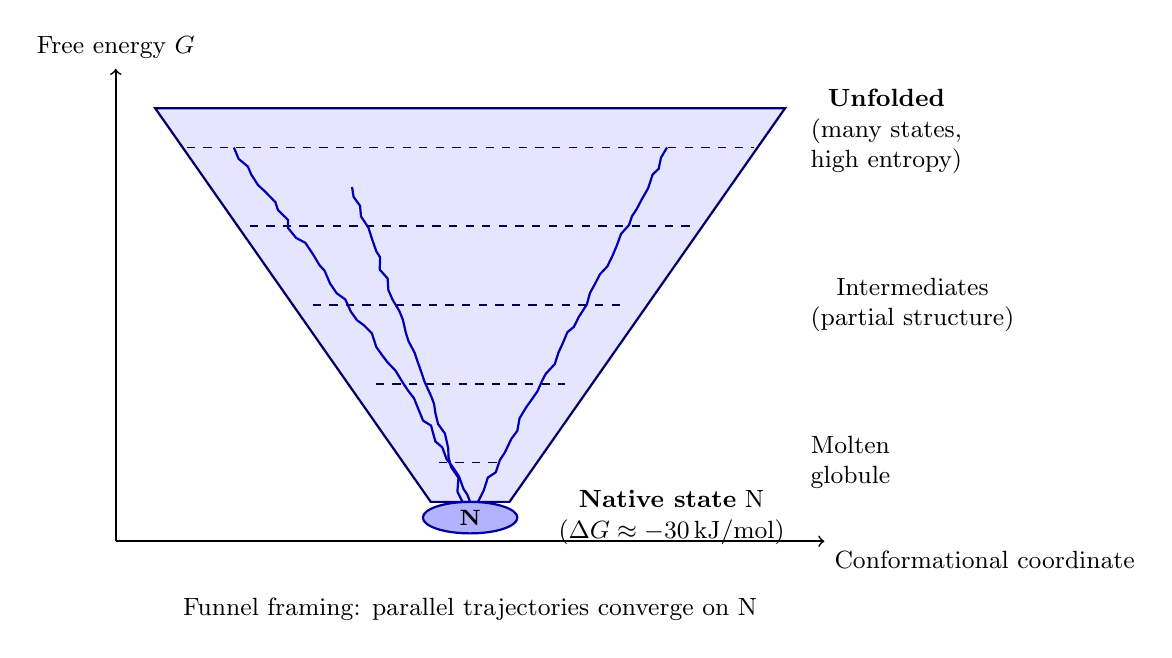
\begin{tikzpicture}[
    funnel/.style={thick, blue!50!black},
    arrow/.style={->, thick, gray},
    label/.style={font=\small, align=center},
]

% Funnel outline: V-shape opening upward.
\filldraw[fill=blue!10, draw=blue!40!black, thick]
    (-4.0, 4.5) -- (-0.5, -0.5) -- (0.5, -0.5) -- (4.0, 4.5) -- cycle;

% Internal contour lines (energy isolines)
\foreach \y/\w in {4.0/3.6, 3.0/2.8, 2.0/2.0, 1.0/1.2, 0.0/0.4}{
  \draw[blue!30!black, dashed, semithick]
      ({-\w}, \y) -- ({\w}, \y);
}

% Native-state basin at the bottom
\draw[blue!60!black, fill=blue!30, thick]
    (0,-0.7) ellipse (0.6 and 0.2);
\node[font=\footnotesize\bfseries] at (0, -0.7) {N};

% Axes
\draw[->, semithick] (-4.5, -1.0) -- (-4.5, 5.0)
    node[above, label] {Free energy $G$};
\draw[->, semithick] (-4.5, -1.0) -- (4.5, -1.0)
    node[below right, label] {Conformational coordinate};

% Sample trajectories
\draw[blue!70!black, thick, decorate, decoration={random steps, segment length=4pt, amplitude=1pt}]
    (-3.0, 4.0) .. controls (-2.0, 2.5) and (-1.0, 1.5) .. (0.0, -0.5);
\draw[blue!70!black, thick, decorate, decoration={random steps, segment length=4pt, amplitude=1pt}]
    (2.5, 4.0) .. controls (1.5, 2.0) and (0.7, 0.7) .. (0.1, -0.5);
\draw[blue!70!black, thick, decorate, decoration={random steps, segment length=4pt, amplitude=1pt}]
    (-1.5, 3.5) .. controls (-0.8, 1.5) and (-0.3, 0.4) .. (-0.1, -0.5);

% Annotations
\node[label, anchor=west] at (4.2, 4.2)
    {\textbf{Unfolded}\\(many states,\\high entropy)};
\node[label, anchor=west] at (4.2, 2.0)
    {Intermediates\\(partial structure)};
\node[label, anchor=west] at (4.2, 0.0)
    {Molten\\globule};
\node[label, anchor=west] at (1.0, -0.7)
    {\textbf{Native state} N\\($\Delta G \approx -30\,$kJ/mol)};

% Levinthal comparison
\node[label, anchor=north] at (0, -1.6)
    {Funnel framing: parallel trajectories converge on N};

\end{tikzpicture}

\caption{The folding-energy landscape, as a funnel. The unfolded
ensemble at the top has many conformations and high entropy; the
native state N at the bottom is a single low-entropy basin.
Trajectories from arbitrary starting points converge on N by
following the energy gradient. The funnel framing replaces
Levinthal's random search with parallel biased motion.}
\label{fig:v6c04-funnel}
\end{figure}

\engterm{Folding intermediates and pathways}. Most proteins fold
through one or more intermediate states. The molten-globule
intermediate has approximately the correct secondary structure but
loose tertiary packing; subsequent steps refine the side-chain
contacts to give the native state. The classical phi-value analysis
of Fersht and others identifies the residues whose stabilising
interactions form early in the folding pathway (the folding nucleus)
versus those that form late \cite{paper:v6c04-fersht-phi-1995}. For
many small proteins, the folding nucleus comprises $5$ to $10$
residues whose hydrophobic core forms in the first few microseconds
and templates the rest of the fold.

\engterm{Chaperones}. The cell's protein-folding machinery includes
families of chaperone proteins that assist folding without becoming
part of the final structure. The Hsp70 family binds nascent
polypeptide chains as they emerge from the ribosome and prevents
premature aggregation; the GroEL/GroES chaperonin system in bacteria
(and the eukaryotic TRiC/CCT system) provides an isolated folding
chamber in which a misfolded protein can attempt folding without
interference from other proteins. The cell's chaperone capacity is
upregulated under heat stress (the heat-shock response), under
oxidative stress, and in cells with high protein-synthesis demand.
Chaperone failure is implicated in many of the misfolding diseases
named in the failure section.

\engterm{Computational structure prediction}. Predicting protein
structure from sequence was a fifty-year challenge that approached
practical resolution in 2020 with DeepMind's AlphaFold 2. The system
achieved approximately experimental-quality accuracy on the CASP14
benchmark (median backbone RMSD of $1\,\si{\angstrom}$ against
crystal-structure references) and has subsequently produced
predicted structures for $\sim 200\,$million proteins in the AlphaFold
database \cite{paper:jumper-alphafold2-2021,paper:v6c04-jumper-alphafold-2021}.
The success has transformed structural biology by making predicted
structures routinely available for proteins that have never been
crystallised. The system's limitations (it predicts a single static
conformation, does not handle most ligand binding well, and is less
reliable for intrinsically disordered regions) remain active research
areas at the time of writing (current as of 2025). The chapter's
\path{code/levinthal_paradox.py} computes the random-search timescale
for protein sizes from $50$ to $250$ residues, alongside the observed
folding-time range, and quantifies the speedup achieved by the funnel
framing.

\begin{principle}[Sequence specifies structure under physiological conditions]
For most proteins, the amino-acid sequence under cellular solvent and
temperature conditions uniquely determines the three-dimensional
fold. The determination is thermodynamic (native state is the
global free-energy minimum) and engineered by selection (the
folding-energy landscape funnels toward the native state on the
timescale of the cell's protein-synthesis rate). The principle
makes possible the engineering programme of designing a desired
function and synthesising a sequence that folds to perform it.
\end{principle}

\section{Enzymes as catalysts}\pathtag{core}

An \engterm{enzyme} is a protein (or, in some cases, an RNA) that
catalyses a specific chemical reaction. Enzymes accelerate reactions
by factors of $10^6$ to $10^{17}$ over the uncatalysed rate, with
rate enhancements concentrated at the chemically difficult steps that
the cell needs to control \cite[ch.~6]{text:lehninger-biochemistry}.

\engterm{Catalytic mechanism}. The enzyme catalyses a reaction by
binding the substrate in a specific orientation (\engterm{transition-state
stabilisation}) and by providing a chemical environment that stabilises
the reaction transition state more than the substrate or product. The
binding pocket (the \engterm{active site}) is a small region of the
protein, usually $1\,\text{nm}^3$ or smaller, lined with the catalytic
amino-acid residues that participate in the reaction. The
transition-state stabilisation lowers the activation energy and so
accelerates the reaction.

\engterm{Michaelis-Menten kinetics}. The rate of an enzyme-catalysed
reaction depends on the substrate concentration in a saturable way
described by the Michaelis-Menten equation
\[
v = \frac{V_{\max} [S]}{K_M + [S]},
\]
where $V_{\max}$ is the maximum rate (saturating substrate), $K_M$
is the Michaelis constant (the substrate concentration at which the
rate is half-maximum), and $[S]$ is the substrate concentration. The
parameter $K_M$ ranges from $10^{-7}$ to $10^{-3}\,\text{M}$ for
typical enzymes and is usually close to the physiological substrate
concentration, so that the enzyme operates in the sensitive
intermediate region of the rate curve. The maximum turnover number
$k_{\text{cat}} = V_{\max} / [E]_{\text{total}}$ ranges from $1$ to
$10^7\,\text{s}^{-1}$. The catalytic efficiency
$k_{\text{cat}}/K_M$ ranges up to $10^9\,\text{M}^{-1}\text{s}^{-1}$;
the upper limit is set by the diffusion-limited encounter rate
between enzyme and substrate, and the most efficient enzymes
(carbonic anhydrase, acetylcholinesterase, triose phosphate isomerase)
operate at or near this limit \cite[ch.~6]{text:lehninger-biochemistry}.
The Michaelis-Menten formalism was derived by Leonor Michaelis and
Maud Menten in 1913 \cite{paper:michaelis-menten1913,paper:v6c04-michaelis-menten-1913};
the modern steady-state form is due to Briggs and Haldane in 1925
\cite{paper:v6c04-briggs-haldane-1925}.

\engterm{Worked example: Michaelis-Menten fit}. The chapter's
\path{data/mm_kinetics_example.csv} carries a synthetic
$v$-versus-$[S]$ dataset generated from $V_{\max} = 46\,\si{\micro\meter}/\text{min}$
and $K_M = 1.2 \times 10^{-4}\,\text{M}$ with $5\%$ multiplicative noise.
Running \path{code/michaelis_menten_fit.py} on the dataset returns
$V_{\max} = 45.9 \pm 0.6\,\si{\micro\meter}/\text{min}$ and
$K_M = (1.19 \pm 0.05) \times 10^{-4}\,\text{M}$, recovering the
generating parameters to within statistical error. The
Lineweaver-Burk linearisation $1/v = (K_M/V_{\max})(1/[S]) + 1/V_{\max}$
gives biased estimates ($V_{\max} \approx 47.5$, $K_M \approx 1.28
\times 10^{-4}\,\text{M}$) because the reciprocal transform inflates
errors at low $[S]$. Nonlinear least squares is the standard of
practice; the Lineweaver-Burk plot survives as a teaching diagnostic.
Figure~\ref{fig:v6c04-mm} plots the hyperbola with the
Lineweaver-Burk inset.

\begin{figure}[ht]
\centering
% Michaelis-Menten v versus [S] hyperbola, with Lineweaver-Burk inset.
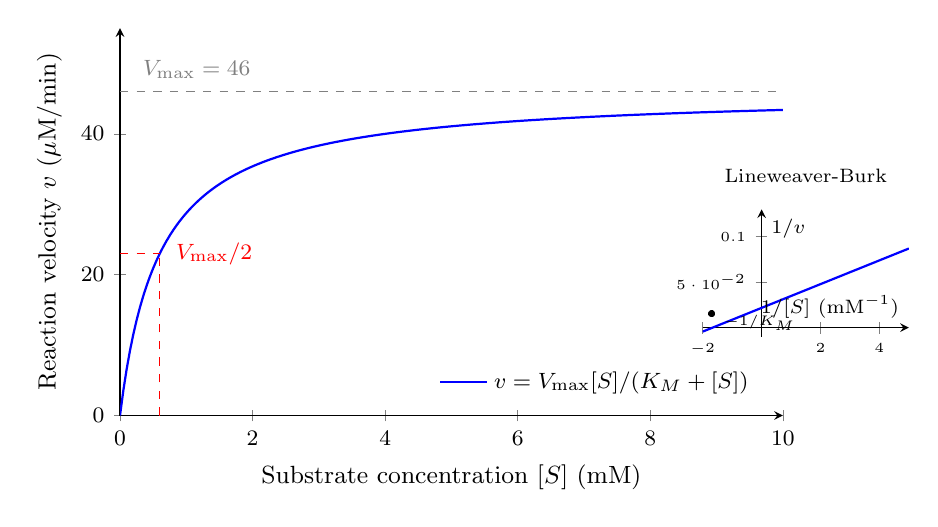
\begin{tikzpicture}
\begin{axis}[
    width=10cm, height=6.5cm,
    xlabel={Substrate concentration $[S]$ (mM)},
    ylabel={Reaction velocity $v$ ($\mu$M/min)},
    domain=0:10,
    samples=200,
    xmin=0, xmax=10,
    ymin=0, ymax=55,
    axis lines=left,
    legend pos=south east,
    legend cell align=left,
    legend style={font=\footnotesize, draw=none},
    every axis label/.append style={font=\small},
    every tick label/.append style={font=\footnotesize},
]
% Main MM curve: Vmax = 46, Km = 0.6 (in mM units to keep numbers tidy)
\addplot[blue, thick, no marks] {46*x/(0.6 + x)};
\addlegendentry{$v = V_{\max}[S]/(K_M + [S])$}

% Vmax asymptote
\addplot[gray, dashed, no marks] coordinates {(0, 46) (10, 46)};
\node[anchor=south west, font=\footnotesize, gray] at (axis cs:0.2, 46.5) {$V_{\max} = 46$};

% Km marker: v = Vmax/2 at S = Km = 0.6
\addplot[red, dashed, no marks] coordinates {(0.6, 0) (0.6, 23)};
\addplot[red, dashed, no marks] coordinates {(0, 23) (0.6, 23)};
\node[anchor=west, font=\footnotesize, red] at (axis cs:0.7, 23) {$V_{\max}/2$};
\node[anchor=north, font=\footnotesize, red] at (axis cs:0.6, -0.5) {$K_M = 0.6$};

\end{axis}

% Lineweaver-Burk inset: 1/v vs 1/[S], straight line
\begin{axis}[
    at={(7.4cm, 1.0cm)},
    anchor=south west,
    width=4.2cm, height=3.2cm,
    xlabel={\scriptsize $1/[S]$ (mM$^{-1}$)},
    ylabel={\scriptsize $1/v$},
    domain=-2:5,
    samples=100,
    xmin=-2, xmax=5,
    ymin=-0.01, ymax=0.13,
    axis lines=middle,
    every axis label/.append style={font=\scriptsize},
    every tick label/.append style={font=\tiny},
    title={\scriptsize Lineweaver-Burk},
    title style={font=\scriptsize},
]
% 1/v = (Km/Vmax)*(1/S) + 1/Vmax = (0.6/46)*x + 1/46
\addplot[blue, thick] {(0.6/46)*x + 1/46};
% x-intercept = -1/Km = -1.67
\node[font=\tiny] at (axis cs:-1.67, 0.015) {\textbullet};
\node[font=\tiny, anchor=west] at (axis cs:-1.6, 0.005) {$-1/K_M$};
\end{axis}

\end{tikzpicture}

\caption{The Michaelis-Menten rate law. Main panel: velocity $v$ as
a function of substrate concentration $[S]$, with $V_{\max}$
asymptote and $K_M$ (the $[S]$ at half-saturation) marked. Inset:
Lineweaver-Burk double-reciprocal linearisation, with the
$x$-intercept giving $-1/K_M$ and the $y$-intercept giving
$1/V_{\max}$.}
\label{fig:v6c04-mm}
\end{figure}

\engterm{Catalytic strategies}. The cell uses six principal
catalytic strategies: \engterm{acid-base catalysis} (proton transfer
to or from the substrate), \engterm{covalent catalysis} (formation of
a temporary covalent enzyme-substrate intermediate), \engterm{metal-ion
catalysis} (a metal cofactor stabilises charge or activates water),
\engterm{electrostatic catalysis} (the enzyme's electrostatic
environment stabilises charged transition states), \engterm{proximity
and orientation} (the enzyme binds the substrate in the geometry
required for reaction), and \engterm{strain induction} (the enzyme
distorts the substrate toward the transition-state geometry). Most
enzymes use several strategies simultaneously; the specific
combination is set by the chemistry of the catalysed reaction.

\engterm{Enzyme classification}. The Enzyme Commission (EC)
classification organises enzymes by reaction type into six main
classes: oxidoreductases (electron transfer reactions),
transferases (group transfer reactions, including kinases that
transfer phosphate), hydrolases (hydrolytic cleavage), lyases
(non-hydrolytic cleavage), isomerases (rearrangements), and ligases
(bond formation coupled to ATP or GTP hydrolysis). The
classification, dating to the International Union of Biochemistry's
1961 report, is the standard engineering vocabulary for the cell's
catalytic catalogue. The chapter's \path{data/enzyme_kinetics.csv}
tabulates $k_{\text{cat}}$, $K_M$, and $k_{\text{cat}}/K_M$ for
ten representative enzymes spanning catalase
($k_{\text{cat}} = 4 \times 10^7\,\text{s}^{-1}$) to RuBisCO
($k_{\text{cat}} = 3.3\,\text{s}^{-1}$). The range of $k_{\text{cat}}$
spans seven orders of magnitude; the range of $k_{\text{cat}}/K_M$
spans only three orders. The narrower spread of catalytic efficiency
reflects the diffusion-limited ceiling.

\section{Allosteric regulation}\pathtag{standard}

The cell needs to regulate enzymatic activity in response to changing
metabolic conditions. The principal mechanism is
\engterm{allosteric regulation}: a molecule binds at a site distinct
from the active site (the \engterm{allosteric site}) and changes the
enzyme's activity by altering its conformation. The mechanism allows
the activity of an enzyme to be modulated by signals that are
chemically unrelated to its substrate.

\engterm{Two canonical models}. The MWC (Monod-Wyman-Changeux) model
of 1965 \cite{paper:v6c04-monod-wyman-changeux-1965} treats an
allosteric enzyme as existing in two conformational states (R,
``relaxed'' or active; T, ``tense'' or inactive) that interconvert
reversibly, with substrate binding shifting the equilibrium toward R.
The KNF (Koshland-N\'emethy-Filmer) model
\cite{paper:v6c04-koshland-1966} treats the conformational change as
occurring sequentially on each subunit upon substrate binding (induced
fit). The two models give different specific predictions for the
cooperativity curves, and many real enzymes are intermediate between
them.

\engterm{Cooperativity and the Hill equation}. Allosteric enzymes
with multiple substrate-binding sites display cooperative binding:
the binding of one substrate molecule alters the affinity for the
next. Positive cooperativity (later sites bind more tightly) gives
the steep sigmoidal binding curve characteristic of haemoglobin
oxygen binding. The empirical Hill equation
\cite{paper:v6c04-hill-1910}
\[
\theta = \frac{[S]^n}{K^n + [S]^n}
\]
parameterises the cooperativity by the Hill coefficient $n$, which
for non-cooperative binding equals $1$, for haemoglobin is
approximately $2.8$, and for the most cooperative natural systems
approaches the number of binding sites $n_{\max}$. The Hill equation
is empirical; the MWC and KNF models give it mechanistic
interpretation.

\engterm{Worked example: haemoglobin oxygen-dissociation curve}. The
chapter's \path{code/hill_cooperativity.py} fits the Hill equation to
the human haemoglobin oxygen-saturation data in
\path{data/hemoglobin_oxygen_binding.csv}, returning
$P_{50} = 26\,\text{mmHg}$ and $n_H = 2.8$. The same fit applied to
myoglobin data (single-site, non-cooperative) returns
$P_{50} = 2.8\,\text{mmHg}$ and $n_H \approx 1$. The cooperative
haemoglobin releases approximately $37\%$ of its bound oxygen
between the lung partial pressure ($\sim 100\,\text{mmHg}$, $Y
\approx 0.97$) and the resting-tissue partial pressure
($\sim 26\,\text{mmHg}$, $Y \approx 0.50$); the non-cooperative
myoglobin releases only $\sim 5\%$ over the same range. Cooperativity
is the engineering means by which the same hemoglobin tetramer
both binds avidly at the lung and releases efficiently at the tissue.
Perutz worked out the structural basis (salt-bridge rearrangement
between the deoxy T and oxy R quaternary states) by X-ray
crystallography in the 1960s and 1970s \cite{paper:v6c04-perutz-1970}.
Figure~\ref{fig:v6c04-hill} plots the two saturation curves.

\begin{figure}[ht]
\centering
% Hill saturation curves for haemoglobin (n approx 2.8) and myoglobin (n approx 1).
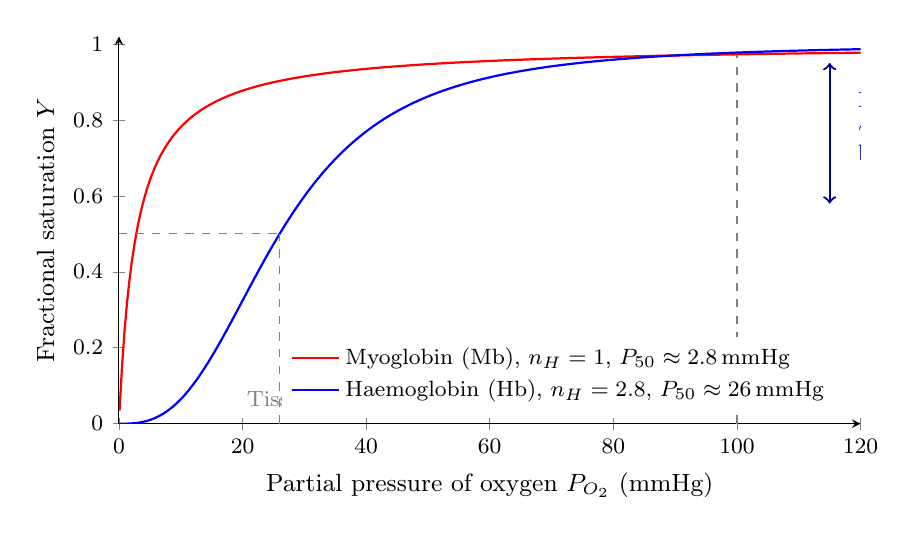
\begin{tikzpicture}
\begin{axis}[
    width=11cm, height=6.5cm,
    xlabel={Partial pressure of oxygen $P_{O_2}$ (mmHg)},
    ylabel={Fractional saturation $Y$},
    domain=0.1:120,
    samples=300,
    xmin=0, xmax=120,
    ymin=0, ymax=1.02,
    axis lines=left,
    legend pos=south east,
    legend cell align=left,
    legend style={font=\footnotesize, draw=none},
    every axis label/.append style={font=\small},
    every tick label/.append style={font=\footnotesize},
]

% Myoglobin: Hill n = 1, P50 = 2.8 mmHg
\addplot[red, thick, no marks] {x^1/(2.8^1 + x^1)};
\addlegendentry{Myoglobin (Mb), $n_H = 1$, $P_{50} \approx 2.8$\,mmHg}

% Haemoglobin: Hill n = 2.8, P50 = 26 mmHg
\addplot[blue, thick, no marks] {x^2.8/(26^2.8 + x^2.8)};
\addlegendentry{Haemoglobin (Hb), $n_H = 2.8$, $P_{50} \approx 26$\,mmHg}

% Tissue P_O2 marker
\addplot[gray, dashed, no marks] coordinates {(26, 0) (26, 0.5)};
\addplot[gray, dashed, no marks] coordinates {(0, 0.5) (26, 0.5)};
\node[anchor=south, font=\footnotesize, gray] at (axis cs:26, 0.02) {Tissue};

% Lung P_O2 marker
\addplot[gray, dashed, no marks] coordinates {(100, 0) (100, 0.97)};
\node[anchor=south, font=\footnotesize, gray] at (axis cs:100, 0.02) {Lung};

% Delivery range arrow for Hb between 100 and 26
\draw[<->, thick, blue!60!black]
    (axis cs:115, 0.95) -- (axis cs:115, 0.58);
\node[anchor=west, font=\footnotesize, blue!60!black, align=left]
    at (axis cs:118, 0.78) {Hb delivers\\$\sim$37\% of\\bound O$_2$};

\end{axis}
\end{tikzpicture}

\caption{Oxygen saturation curves for haemoglobin (cooperative,
$n_H \approx 2.8$, $P_{50} \approx 26\,\text{mmHg}$) and myoglobin
(non-cooperative, $n_H \approx 1$, $P_{50} \approx 2.8\,\text{mmHg}$).
The dashed verticals mark the lung and tissue partial pressures.
Cooperativity converts a $4\times$ change in $P_{O_2}$ into a
$2\times$ change in saturation; the non-cooperative myoglobin
changes only marginally over the same range.}
\label{fig:v6c04-hill}
\end{figure}

\engterm{MWC parameters of haemoglobin}. In the MWC framework the
haemoglobin tetramer is described by the allosteric equilibrium
constant $L = [T_0]/[R_0] \approx 9000$ and the affinity ratio
$c = K_R / K_T \approx 0.014$. The script
\path{code/mwc_allostery.py} computes the Hill coefficient as a
function of $(L, c)$ and confirms that these values reproduce the
observed $n_H \approx 2.8$. The MWC framework gives the Hill
coefficient a mechanistic reading: $n_H$ is set by the steepness of
the T-to-R transition, not by the number of binding sites alone.
Effectors that bind preferentially to the T state (2,3-bisphosphoglycerate,
H$^+$, CO$_2$) increase $L$ and shift the curve right, supporting
oxygen release in the tissues; effectors that bind R (CO) decrease
the effective $L$ and shift the curve left, supporting toxicity at low
oxygen partial pressure.

\engterm{Feedback inhibition}. The cell uses allosteric regulation to
build feedback loops at the enzyme level. The end product of a
biosynthetic pathway often binds allosterically to the pathway's
first enzyme and inhibits it; when the end product accumulates, the
pathway shuts down. The bacterial aspartate transcarbamylase (ATCase)
in pyrimidine biosynthesis is the textbook example: the end product
CTP binds at a site distant from the active site and reduces the
enzyme's substrate affinity. The feedback loop is one of the cell's
fastest regulatory mechanisms (response time of seconds to minutes,
compared to hours for transcriptional regulation) and is the
mechanism of choice for stabilising biosynthetic-pathway fluxes
against perturbations.

\engterm{Covalent modification as a control variable}. Many enzymes
are regulated by reversible covalent modification of a specific
amino acid residue. Phosphorylation of serine, threonine, or
tyrosine residues by protein kinases is the most common modification;
the modification is reversed by phosphatases. Phosphorylation
changes the enzyme's activity, its subcellular localisation, or its
binding partners. The kinase-phosphatase network of a typical
mammalian cell contains $\sim 500$ kinases and $\sim 200$
phosphatases and constitutes a major fraction of the cell's
regulatory bandwidth.

\engterm{The dissociation constant $K_d$}. Binding affinity is the
common currency of allosteric regulation, ligand-receptor pharmacology,
and antibody recognition. For a one-to-one binding equilibrium
$P + L \rightleftharpoons PL$ at concentrations well below the
free-protein concentration, the dissociation constant is
\[
K_d = \frac{[P][L]}{[PL]},
\]
the ligand concentration at half-saturation of the protein. A
$K_d$ of $10^{-9}\,\text{M}$ (nanomolar) is typical of strong
antibody-antigen pairs and tight pharmacological inhibitors;
$10^{-6}\,\text{M}$ (micromolar) is typical of substrate-enzyme
binding; $10^{-3}\,\text{M}$ (millimolar) is typical of weak
metabolic interactions. The $K_d$ is related to the binding free
energy by $\Delta G^{\circ} = -RT \ln(1/K_d)$, so each tenfold
improvement in $K_d$ corresponds to $\sim 6\,\text{kJ}/\text{mol}$
of additional binding energy. The nanomolar-to-millimolar range of
$K_d$ values therefore spans $\sim 35\,\text{kJ}/\text{mol}$, the
budget within which single-residue substitutions and small-molecule
modifications operate.

\section{Motor proteins}\pathtag{standard}

The cell uses ATP-hydrolysing motor proteins for directed motion at
the molecular scale. The motor proteins are organised into three
principal families that walk along cytoskeletal tracks:
\engterm{myosin} on actin filaments, \engterm{kinesin} on microtubules
toward the plus end, and \engterm{dynein} on microtubules toward the
minus end. A fourth class, the \engterm{rotary motors} (the
mitochondrial ATP synthase, the bacterial flagellar motor), perform
rotational rather than linear motion. The engineering of motor
proteins is treated in detail by Howard
\cite[ch.~5--10]{text:howard-mechanics-motor-proteins,text:v6c04-howard-motor-2001}.

\engterm{Myosin}. The myosin family includes the muscle myosin II
that powers skeletal muscle contraction, the unconventional myosin I
that pulls membrane vesicles along actin filaments, and the myosin V
that walks processively along actin carrying cargo. Each myosin
molecule has a globular head domain that binds actin and hydrolyses
ATP, a neck region (the lever arm), and a tail that determines the
specific function (filament assembly in muscle myosin, cargo binding
in transport myosins). The mechanical work per ATP hydrolysed is
approximately $5\,\text{pN} \times 5\,\text{nm} = 25\,\text{pN} \cdot
\text{nm} = 6\,k_B T$ at $310\,\si{\kelvin}$, or about $25\,\%$ of the
$30\,\text{pN} \cdot \text{nm}$ of free energy available per ATP
under physiological conditions. The mechanical efficiency is
comparable to a well-engineered macroscopic engine. The
single-molecule measurements of myosin step size and stall force
were performed by Finer, Simmons, and Spudich in 1994 using optical
traps \cite{paper:v6c04-finer-simmons-spudich-1994}.
Figure~\ref{fig:v6c04-myosin} sketches the four-state cycle.

\begin{figure}[ht]
\centering
% Myosin cross-bridge cycle: 4 states around a loop.
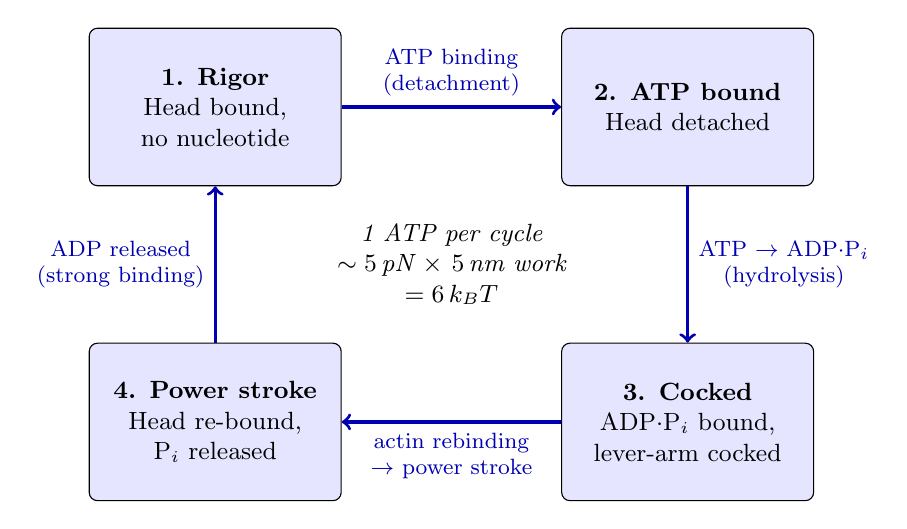
\begin{tikzpicture}[
    state/.style={draw, rounded corners=3pt, fill=blue!10,
                  minimum width=3.2cm, minimum height=2.0cm,
                  align=center, font=\small},
    arr/.style={->, very thick, blue!70!black},
    label/.style={font=\footnotesize, align=center},
]

% Four states arranged in a 2x2 grid
\node[state] (S1) at (0, 4) {\textbf{1. Rigor}\\Head bound,\\no nucleotide};
\node[state] (S2) at (6, 4) {\textbf{2. ATP bound}\\Head detached};
\node[state] (S3) at (6, 0) {\textbf{3. Cocked}\\ADP$\cdot$P$_i$ bound,\\lever-arm cocked};
\node[state] (S4) at (0, 0) {\textbf{4. Power stroke}\\Head re-bound,\\P$_i$ released};

% Arrows around the cycle
\draw[arr] (S1) -- (S2) node[midway, above, label] {ATP binding\\(detachment)};
\draw[arr] (S2) -- (S3) node[midway, right, label] {ATP $\to$ ADP$\cdot$P$_i$\\(hydrolysis)};
\draw[arr] (S3) -- (S4) node[midway, below, label] {actin rebinding\\$\to$ power stroke};
\draw[arr] (S4) -- (S1) node[midway, left, label] {ADP released\\(strong binding)};

% Cycle annotation in centre
\node[align=center, font=\small\itshape] at (3, 2)
    {1 ATP per cycle\\$\sim 5\,$pN $\times$ $5\,$nm work\\$= 6\,k_BT$};

\end{tikzpicture}

\caption{Myosin cross-bridge cycle. State 1 (rigor): head bound to
actin with no nucleotide. State 2: ATP binding detaches the head.
State 3: ATP hydrolysis cocks the lever arm. State 4: head rebinds
actin and executes the power stroke as P$_i$ is released. One ATP
per cycle, $\sim 6\,k_B T$ of work delivered.}
\label{fig:v6c04-myosin}
\end{figure}

\engterm{Muscle contraction}. Skeletal muscle is a particularly
well-characterised example. The contractile unit is the
\engterm{sarcomere}, a $2\,\si{\micro\meter}$-long structure
consisting of interdigitated thin (actin) and thick (myosin)
filaments. The myosin heads project from the thick filaments and bind
the thin filaments; ATP-driven conformational changes in the heads
slide the thin filaments relative to the thick filaments, shortening
the sarcomere. The sliding-filament model
\cite{paper:v6c04-huxley-niedergerke-1954,paper:v6c04-huxley-hanson-1954}
is the canonical mechanism. A single muscle cell contains thousands
of sarcomeres in series within each myofibril and thousands of
myofibrils in parallel; the macroscopic force is the integral over
the parallel myofibrils, and the macroscopic shortening is the
integral over the series sarcomeres. The maximum force per
cross-sectional area of skeletal muscle is approximately
$0.3\,\text{MPa}$, set by the density of myosin heads and the
per-head force.

\engterm{Kinesin and dynein}. The kinesin family transports cargo
along microtubules. The dimeric kinesin-1 takes $8\,\text{nm}$ steps
along the microtubule lattice, hydrolysing one ATP per step and
producing forces up to $7\,\text{pN}$
\cite{paper:v6c04-svoboda-block-1993}. The processivity (the
expected number of steps before detachment) is $\sim 100$ for
kinesin-1, giving a typical run length of $1\,\si{\micro\meter}$.
The motor's hand-over-hand stepping mechanism, in which the two
heads alternate between bound and detached states, gives kinesin
the highly processive behaviour required for long-distance cargo
transport in neurons. Dynein operates similarly but in the opposite
direction along the microtubule. Figure~\ref{fig:v6c04-kinesin}
sketches the head-over-head step.

\begin{figure}[ht]
\centering
% Kinesin hand-over-hand stepping along a microtubule.
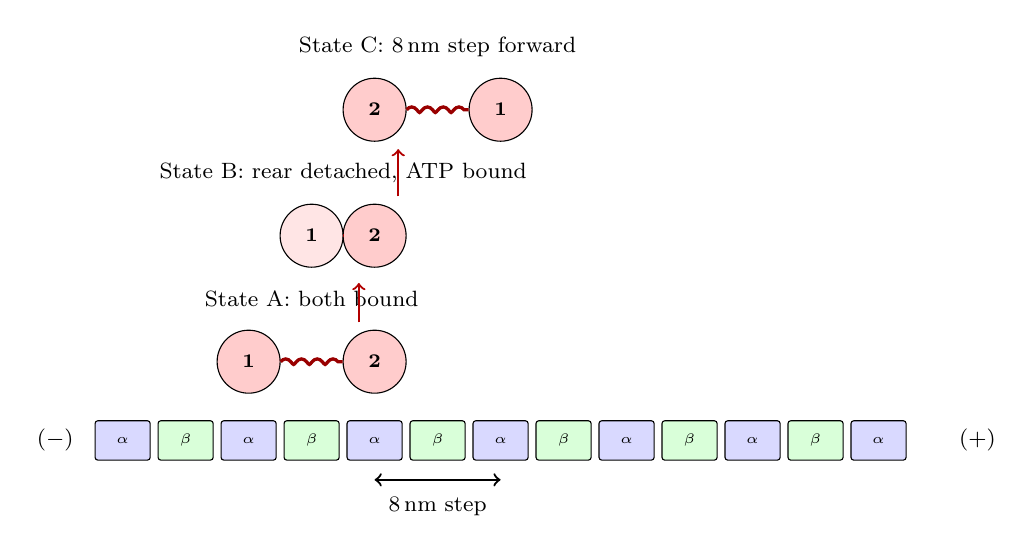
\begin{tikzpicture}[
    tubulin/.style={draw, rounded corners=1pt, minimum width=0.7cm,
                    minimum height=0.5cm, font=\tiny},
    alphat/.style={tubulin, fill=blue!15},
    betat/.style={tubulin, fill=green!15},
    head/.style={circle, draw, fill=red!20, minimum size=8mm, font=\scriptsize\bfseries},
    coil/.style={very thick, red!60!black, decorate,
                 decoration={coil, aspect=0.4, segment length=2mm, amplitude=1pt}},
    arr/.style={->, thick, red!70!black},
]

% Microtubule lattice: alternating alpha and beta tubulin, 8 nm period
\foreach \i in {0,...,12}{
  \pgfmathtruncatemacro{\j}{mod(\i,2)}
  \ifnum\j=0
    \node[alphat] at ({0.8*\i}, 0) {$\alpha$};
  \else
    \node[betat] at ({0.8*\i}, 0) {$\beta$};
  \fi
}
\node[anchor=west, font=\footnotesize] at (10.5, 0) {(+)};
\node[anchor=east, font=\footnotesize] at (-0.5, 0) {($-$)};

% State A: both heads bound (residence)
\node[head] (HA1) at (1.6, 1.0) {1};
\node[head] (HA2) at (3.2, 1.0) {2};
\draw[coil] (HA1) -- (HA2);
\node[font=\footnotesize] at (2.4, 1.8) {State A: both bound};

% State B: rear head detached, leading head pivots
\node[head, fill=red!10] (HB1) at (2.4, 2.6) {1};
\node[head] (HB2) at (3.2, 2.6) {2};
\draw[coil] (HB1) -- (HB2);
\node[font=\footnotesize] at (2.8, 3.4) {State B: rear detached, ATP bound};

% State C: rear head swings forward, binds beta tubulin 8 nm ahead
\node[head] (HC2) at (3.2, 4.2) {2};
\node[head] (HC1) at (4.8, 4.2) {1};
\draw[coil] (HC2) -- (HC1);
\node[font=\footnotesize] at (4.0, 5.0) {State C: 8\,nm step forward};

% Arrows showing progression
\draw[arr] (3.0, 1.5) -- (3.0, 2.0);
\draw[arr] (3.5, 3.1) -- (3.5, 3.7);

% Step size annotation
\draw[<->, thick] (3.2, -0.5) -- (4.8, -0.5);
\node[font=\footnotesize, anchor=north] at (4.0, -0.6) {$8\,$nm step};

\end{tikzpicture}

\caption{Kinesin hand-over-hand stepping on a microtubule. The
$\alpha\beta$-tubulin lattice has an $8\,\text{nm}$ period; each ATP
hydrolysis advances the trailing head by $16\,\text{nm}$ (one full
step) so that the centre of mass advances by $8\,\text{nm}$ per ATP.
A processivity of $\sim 100$ steps gives a $\sim 1\,\si{\micro\meter}$
run length before detachment.}
\label{fig:v6c04-kinesin}
\end{figure}

\engterm{Worked example: kinesin step size and stall force}. The
chapter's \path{code/motor_protein_stall_force.py} implements the
linear force-velocity relation $v(F) = v_0 (1 - F/F_{\text{stall}})$
of \cite{paper:v6c04-howard-1996} alongside the Bell-model
exponential $v(F) = v_0 \exp(-F \delta / k_B T)$ for the near-stall
regime \cite{paper:v6c04-bell-1978}. For kinesin-1 with
$v_0 = 0.8\,\si{\micro\meter}/\text{s}$,
$F_{\text{stall}} = 7\,\text{pN}$, and characteristic load distance
$\delta = 1.3\,\text{nm}$, the linear regime gives
$v = 0.46\,\si{\micro\meter}/\text{s}$ at $3\,\text{pN}$ external
load and $0$ at $7\,\text{pN}$; the Bell model gives $v = 0.32$ and
$0.09\,\si{\micro\meter}/\text{s}$ respectively, capturing the
slow-but-nonzero behaviour observed near stall. The mechanical work
per step at zero load is $7\,\text{pN} \times 8\,\text{nm} =
56\,\text{pN}\cdot\text{nm} \approx 14\,k_B T$, of which only
$6\,k_B T$ is delivered as net forward work because the Brownian
fluctuations of the motor head against the load consume the
remainder. The single-step efficiency is the engineering reading of
why processive motors run at high force but low absolute power.

\engterm{Rotary motors: ATP synthase}. The mitochondrial ATP synthase
(F$_1$F$_0$ ATPase) is a rotary molecular machine that synthesises
ATP from ADP and inorganic phosphate using the proton-motive force
across the mitochondrial inner membrane. The membrane-embedded F$_0$
sector contains a ring of $8$ to $15$ c-subunits that rotate as
protons pass through; the soluble F$_1$ sector contains three
catalytic $\beta$-subunits that synthesise ATP in turn as the
central stalk rotates. The motor was visualised in single-molecule
experiments by Hiroyuki Noji and colleagues in 1997 by attaching an
actin filament to the central stalk and watching it rotate
\cite{paper:v6c04-noji-1997}. The rotation rate is
$\sim 100\,\text{revolutions}/\text{s}$ at full load in mitochondria;
the mechanical work per revolution is three ATP synthesised, or
approximately $200\,\text{pN}\cdot\text{nm}$ of free energy stored
in chemical form. Figure~\ref{fig:v6c04-atpsynthase} sketches the
rotary mechanism.

\begin{figure}[ht]
\centering
% ATP synthase rotary mechanism: F1 (catalytic) and F0 (membrane) sectors.
\begin{tikzpicture}[
    membrane/.style={fill=yellow!20, draw=yellow!40!black},
    beta/.style={draw, rounded corners=4pt, fill=blue!15, minimum width=1.8cm,
                 minimum height=1.5cm, font=\small\bfseries},
    alpha/.style={draw, rounded corners=4pt, fill=blue!10, minimum width=1.8cm,
                 minimum height=1.5cm, font=\small},
    c-ring/.style={draw, fill=green!20, ultra thick},
    stalk/.style={ultra thick, gray!50!black},
    label/.style={font=\footnotesize, align=center},
    arr/.style={->, very thick, red!60!black},
]

% Membrane band
\fill[membrane] (-3.5, 0) rectangle (3.5, 1.8);
\node[label] at (-4.0, 0.9) {membrane};

% F0 c-ring in the membrane
\draw[c-ring] (0, 0.9) ellipse (1.4 and 0.8);
\foreach \i in {0,45,90,135,180,225,270,315}{
  \draw[c-ring] ({1.4*cos(\i)}, {0.9 + 0.8*sin(\i)})
    -- ({1.4*cos(\i+22.5)}, {0.9 + 0.8*sin(\i+22.5)});
}
\node[font=\small, anchor=west] at (1.5, 0.9) {F$_0$};

% Central stalk (gamma subunit) running upward
\draw[stalk] (0, 0.9) -- (0, 4.5);

% F1 head: three alpha-beta pairs around the stalk
\node[alpha] at (-2.0, 4.5) {$\alpha$};
\node[beta] at (-2.0, 6.2) {$\beta$};
\node[alpha] at (0, 6.7) {$\alpha$};
\node[beta] at (0, 5.0) {$\beta$};
\node[alpha] at (2.0, 4.5) {$\alpha$};
\node[beta] at (2.0, 6.2) {$\beta$};

% Catalytic ATP synthesis arrow
\node[anchor=west, align=left] at (3.0, 5.5) {$\beta$ catalyses\\ADP + P$_i$ $\to$ ATP};

% Proton flow arrows (from outside, through F0, to inside)
\node[label, anchor=east] at (-3.7, 2.5) {H$^+$\\(intermembrane)};
\draw[arr] (-3.5, 2.4) -- (-1.5, 1.9);
\draw[arr] (-1.0, 1.5) -- (-0.2, 1.0);
\node[label, anchor=east] at (-3.7, -0.4) {H$^+$\\(matrix)};
\draw[arr] (0.2, 0.7) -- (-1.5, 0.2);
\draw[arr] (-2.0, 0.0) -- (-3.5, -0.3);

% Rotation indicator
\draw[->, thick, red, decoration={markings, mark=at position 0.5 with {\arrow{>}}}]
    (0.7, 4.0) arc (0:340:0.7);
\node[font=\footnotesize, red, anchor=west] at (0.8, 4.0) {$\gamma$ rotation};

% Stoichiometry note
\node[label, anchor=south] at (0, -1.0)
    {$\sim 10$ H$^+$ per revolution; 3 ATP synthesised per revolution.};

\end{tikzpicture}

\caption{ATP synthase rotary mechanism. The membrane-embedded F$_0$
c-ring rotates as protons cross from the intermembrane space to the
matrix; the central $\gamma$ stalk transmits torque to the F$_1$
head, where the three $\beta$ subunits synthesise ATP in turn. The
stoichiometry is $\sim 10$ H$^+$ per revolution and $3$ ATP per
revolution, giving $\sim 3.3$ H$^+$ per ATP.}
\label{fig:v6c04-atpsynthase}
\end{figure}

\engterm{Rotary motors: bacterial flagellum}. The bacterial flagellar
motor rotates at $100$ to $300\,\text{Hz}$ and propels the cell at
$20$ to $50\,\si{\micro\meter}/\text{s}$. The motor uses the proton
gradient across the cell membrane as its energy source (in
\emph{E.~coli}; in marine bacteria it uses sodium gradient).
Approximately $1000$ protons pass through the motor per revolution.
The motor switches direction in response to chemotactic signals from
the cell, producing the run-and-tumble swimming pattern of
\emph{E.~coli} chemotaxis (Chapter~\ref{vol06:ch01}).

\section{Membrane proteins, channels, and pumps}\pathtag{standard}

The plasma membrane (Chapter~\ref{vol06:ch01}) is a lipid bilayer
into which proteins are embedded that perform the membrane's
transport, signalling, and adhesion functions. The principal classes
of membrane protein are channels (passive conductors of ions or
small molecules), pumps (active transporters powered by ATP or a
gradient), receptors (signal transducers), and transporters
(carriers that translocate substrates by conformational change).

\engterm{Ion channels}. Channels conduct ions down their
electrochemical gradient at rates of $10^6$ to $10^8\,\text{ions}/
\text{second}$. The selectivity of a channel (whether it conducts
sodium, potassium, calcium, chloride, or some combination) is set by
a narrow region of the channel pore lined with chemical groups that
discriminate among the candidates by size and charge. The classic
example is the potassium channel selectivity filter, whose backbone
carbonyls mimic the hydration shell of a potassium ion at the cost
that a sodium ion (smaller, with stronger hydration) cannot fit
without paying a large desolvation energy
\cite{paper:v6c04-doyle-kcsa-1998}. The selectivity is typically
$1000:1$ or better; the engineering of the filter is the canonical
example of size-and-coordination-based selectivity in biology
\cite[ch.~14]{text:hille-ion-channels,text:v6c04-hille-channels-2001}.

Channels are gated by various mechanisms: voltage-gated channels
respond to membrane potential changes (the sodium and potassium
channels of the action potential, Chapter~\ref{vol06:ch07});
ligand-gated channels respond to bound chemical signals (the
nicotinic acetylcholine receptor at neuromuscular junctions);
mechano-gated channels respond to membrane stretch (the touch
receptors); temperature-gated channels respond to thermal stimuli
(the TRP channels involved in pain and temperature sensation). The
gating mechanism determines the channel's role in cellular
signalling. Voltage-gated channels in particular cycle through three
states (closed, open, inactivated); the inactivation step underlies
the refractory period of the action potential.
Figure~\ref{fig:v6c04-channel} sketches the three states.

\begin{figure}[ht]
\centering
% Voltage-gated ion channel in three states: closed, open, inactivated.
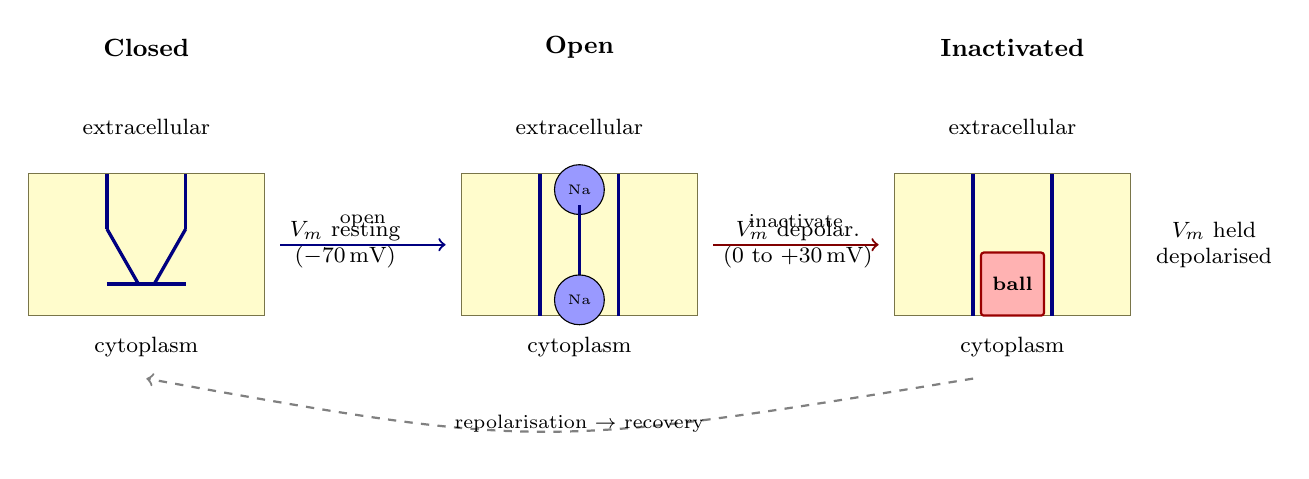
\begin{tikzpicture}[
    membrane/.style={fill=yellow!20, draw=yellow!40!black},
    pore/.style={very thick, blue!50!black},
    block/.style={fill=red!30, draw=red!60!black, thick, rounded corners=1pt},
    label/.style={font=\footnotesize, align=center},
    title/.style={font=\small\bfseries, align=center},
]

% Three panels side by side
% --- CLOSED ---
\begin{scope}[shift={(0,0)}]
\node[title] at (1.5, 3.4) {Closed};
\fill[membrane] (0, 0) rectangle (3, 1.8);
% Outer face
\draw[pore] (1.0, 1.8) -- (1.0, 1.1);
\draw[pore] (2.0, 1.8) -- (2.0, 1.1);
% Inner closed (pore pinched)
\draw[pore] (1.0, 1.1) -- (1.4, 0.4);
\draw[pore] (2.0, 1.1) -- (1.6, 0.4);
\draw[pore] (1.0, 0.4) -- (2.0, 0.4);
% Outside / inside labels
\node[label] at (1.5, 2.4) {extracellular};
\node[label] at (1.5, -0.4) {cytoplasm};
\node[label, anchor=west] at (3.2, 0.9) {$V_m$ resting\\($-70\,$mV)};
\end{scope}

% --- OPEN ---
\begin{scope}[shift={(5.5,0)}]
\node[title] at (1.5, 3.4) {Open};
\fill[membrane] (0, 0) rectangle (3, 1.8);
\draw[pore] (1.0, 1.8) -- (1.0, 0.0);
\draw[pore] (2.0, 1.8) -- (2.0, 0.0);
% Ion arrows
\node[circle, fill=blue!40, draw, minimum size=3mm, font=\tiny] at (1.5, 1.6) {Na};
\draw[->, blue!50!black, thick] (1.5, 1.4) -- (1.5, 0.4);
\node[circle, fill=blue!40, draw, minimum size=3mm, font=\tiny] at (1.5, 0.2) {Na};
\node[label] at (1.5, 2.4) {extracellular};
\node[label] at (1.5, -0.4) {cytoplasm};
\node[label, anchor=west] at (3.2, 0.9) {$V_m$ depolar.\\ (0 to $+30\,$mV)};
\end{scope}

% --- INACTIVATED ---
\begin{scope}[shift={(11,0)}]
\node[title] at (1.5, 3.4) {Inactivated};
\fill[membrane] (0, 0) rectangle (3, 1.8);
\draw[pore] (1.0, 1.8) -- (1.0, 0.0);
\draw[pore] (2.0, 1.8) -- (2.0, 0.0);
% Inactivation ball plug at inner mouth
\node[block, minimum size=8mm] at (1.5, 0.4) {};
\node[label, font=\scriptsize\bfseries] at (1.5, 0.4) {ball};
\node[label] at (1.5, 2.4) {extracellular};
\node[label] at (1.5, -0.4) {cytoplasm};
\node[label, anchor=west] at (3.2, 0.9) {$V_m$ held\\depolarised};
\end{scope}

% Transition arrows
\draw[->, thick, blue!50!black] (3.2, 0.9) -- (5.3, 0.9);
\node[font=\scriptsize, anchor=south] at (4.25, 1.0) {open};
\draw[->, thick, red!50!black] (8.7, 0.9) -- (10.8, 0.9);
\node[font=\scriptsize, anchor=south] at (9.75, 1.0) {inactivate};
\draw[->, thick, gray, dashed] (12.0, -0.8) .. controls (6.5, -1.7) .. (1.5, -0.8);
\node[font=\scriptsize, anchor=south] at (7.0, -1.6) {repolarisation $\to$ recovery};

\end{tikzpicture}

\caption{Voltage-gated ion channel in its three gating states. At
resting potential the channel is closed (pore constricted). On
depolarisation the voltage sensor opens the channel and ions flow
down the electrochemical gradient. Continued depolarisation drives
the inactivation gate (an N-terminal ``ball'') into the inner mouth,
blocking conduction. Repolarisation allows recovery from inactivation.}
\label{fig:v6c04-channel}
\end{figure}

\engterm{Pumps}. Active transporters use an energy input (ATP or a
gradient) to move substrates against their electrochemical gradient.
The sodium-potassium ATPase (Chapter~\ref{vol06:ch01}) is the
canonical example: it exchanges $3\,\text{Na}^+$ outward for
$2\,\text{K}^+$ inward per ATP hydrolysed, against both ions'
gradients \cite{paper:v6c04-skou-1957}. The Ca$^{2+}$-ATPase pumps
$2\,\text{Ca}^{2+}$ per ATP out of the cytoplasm into intracellular
compartments. The H$^+$-ATPases acidify lysosomes and the plant
vacuole. The cell's energy budget for these pumps is large: the
sodium-potassium ATPase alone consumes $20\,\%$ to $30\,\%$ of the
cell's resting ATP supply in many neurons.

\engterm{Transporters}. Carriers translocate substrates by undergoing
conformational changes that alternately expose the binding site to
one side of the membrane and the other. The glucose transporter
GLUT1 is the textbook example: it binds glucose on the extracellular
side, undergoes a conformational change to expose the binding site
to the cytoplasm, releases glucose, returns to the original
conformation, and repeats. The transport rate is approximately
$1000\,\text{glucose}/\text{transporter}/\text{s}$, slower than ion
channels by three to four orders of magnitude. The slower rate is
the price the cell pays for the conformational-change mechanism
that handles polar molecules too large for simple channel passage.

\engterm{Receptors}. Membrane receptors transduce extracellular
signals into intracellular responses. The principal classes are
G-protein-coupled receptors (GPCRs, $\sim 800$ in the human genome),
receptor tyrosine kinases (the insulin receptor, growth-factor
receptors), ion-channel receptors (the nicotinic acetylcholine
receptor), and intracellular receptors that bind lipid-soluble ligands
(steroid hormone receptors). The GPCRs are the most diverse class
and the target of approximately $30\,\%$ of currently approved
pharmaceuticals (current as of 2024).

\begin{archetype}[Control and scaling at the molecular machine]
The protein machines of the cell exhibit the control and scaling
archetypes. The control archetype: enzymes are controlled by
allosteric regulators and by covalent modification with response
times of seconds to minutes; ion channels are controlled by voltage,
ligand, and mechanical signals with response times of microseconds
to milliseconds; motor proteins are controlled by the local availability
of ATP and by regulatory binding partners. The scaling archetype:
proteins span four orders of magnitude in mass (from short peptides at
$10^3\,\text{Da}$ to large multi-subunit complexes at
$10^7\,\text{Da}$) with consistent engineering principles applying
across the range. The ribosome, at $2.5$ to $4\,\text{MDa}$, performs
the same template-driven polymer synthesis as a single small enzyme
does in catalysing a single reaction; the architecture scales.
\end{archetype}

\begin{estimation}
\textbf{Question.} Estimate the number of myosin heads engaged
simultaneously with actin filaments in a single fully contracted
human biceps muscle.

\smallskip
\textit{Estimate, before reading on.}

\smallskip
A human biceps muscle has a physiological cross-section of
approximately $30\,\text{cm}^2 = 3 \times 10^{-3}\,\text{m}^2$ at
adult maximum. The maximum force per cross-sectional area is
approximately $0.3\,\text{MPa}$, giving a maximum tendon force of
$900\,\text{N}$. The force per engaged myosin head is approximately
$5\,\text{pN} = 5 \times 10^{-12}\,\text{N}$.

The number of simultaneously engaged myosin heads is the muscle force
divided by the per-head force:
\[
N_{\text{heads}} = \frac{900}{5 \times 10^{-12}} = 1.8 \times 10^{14}.
\]

Cross-check from sarcomere geometry: a sarcomere is
$2\,\si{\micro\meter}$ long with approximately $300$ myosin heads
projecting from each thick filament; the biceps cross-section
contains approximately $10^9$ thick filaments (areal density of
$\sim 3 \times 10^{11}/\text{m}^2$ times $3 \times 10^{-3}\,\text{m}^2$).
Total heads in the cross-section is $3 \times 10^{11}$. With a typical
duty cycle of $30\,\%$ to $50\,\%$ of heads engaged at any moment, the
engaged-heads count is $\sim 10^{11}$.

\smallskip
\textit{Postmortem.} The two estimates differ by a factor of
$\sim 10^3$. The first estimate assumes that every myosin head in the
muscle contributes simultaneously, which overcounts because only a
single layer of heads at each thick filament is engaged at one
instant (the heads are spaced along the filament length and engage
sequentially) and only $30\,\%$ to $50\,\%$ of those are bound at any
moment. Applying both corrections to the first estimate brings it
within a factor of five of the geometric estimate. The remaining
discrepancy traces to the per-head force, which varies between
$3\,\text{pN}$ in low-load conditions and $10\,\text{pN}$ at peak
isometric contraction. The two estimates agree to within the
uncertainty of those parameters. The exercise illustrates the
order-of-magnitude character of biological scaling: the number of
engaged motor proteins in a macroscopic action is $\sim 10^{11}$, a
number that is large in absolute terms but small relative to the
total myosin-head inventory.
\end{estimation}

\begin{estimation}
\textbf{Question.} Estimate the rotation rate of mitochondrial ATP
synthase in a resting human cell from the cellular ATP turnover rate.

\smallskip
\textit{Estimate, before reading on.}

\smallskip
A resting adult consumes ATP at a rate of approximately
$65\,\text{kg/day}$ of ATP (the body weight in ATP turnover per day,
a common biochemistry benchmark). At $507\,\text{g/mol}$, that is
$1.3 \times 10^{2}\,\text{mol}$ ATP per day, or
$7.4 \times 10^{19}$ ATP molecules per second across the whole body.
The body contains approximately $3 \times 10^{13}$ cells, so the
per-cell ATP turnover is $\sim 2.5 \times 10^{6}$ ATP/s. Each cell
contains approximately $1000$ to $2000$ mitochondria, and each
mitochondrion contains approximately $10^4$ ATP synthase copies
(the inner-membrane density is $\sim 10^4$ ATPase per
$\si{\micro\meter}^2$ and the cristae surface area per mitochondrion
is $\sim 1\,\si{\micro\meter}^2$). Total ATP synthase per cell is
$\sim 10^7$. Each ATP synthase rotation produces three ATP, so the
required per-synthase rotation rate is
\[
\nu = \frac{2.5 \times 10^{6}\,\text{ATP/s}}{10^7 \times 3\,\text{ATP/rev}}
\approx 0.1\,\text{rev/s}.
\]

\textit{Cross-check from in-vitro single-molecule measurements.} Noji
and colleagues observed in-vitro rotation rates of
$\sim 130\,\text{rev/s}$ at saturating substrate concentrations
\cite{paper:v6c04-noji-1997}. The in-vivo resting rate is approximately
three orders of magnitude lower, consistent with the engine running
well below its peak turnover under resting conditions.

\smallskip
\textit{Postmortem.} The estimate has two large uncertainties: the
per-cell mitochondrial inventory varies from approximately $200$ (in
lymphocytes) to $> 10^4$ (in cardiomyocytes), and the per-mitochondrion
ATP synthase copy number varies with the cristae surface area. A
cardiomyocyte at peak load might run its ATP synthases at $\sim 30$
to $50\,\text{rev/s}$; a resting lymphocyte at
$\sim 0.01\,\text{rev/s}$. The order-of-magnitude estimate
identifies the resting set point; the four-order-of-magnitude
headroom is the engineering reading of why the mitochondrion can
ramp ATP output rapidly under exercise.
\end{estimation}

\section{Failure: misfolding diseases}\pathtag{core}

Proteins fail by misfolding. Misfolding is a chemically benign event
when a single protein molecule fails to reach its native fold and is
degraded; it becomes pathological when misfolded proteins accumulate,
aggregate, or evade degradation. The section names four mechanism
classes of protein-misfolding disease (amyloid aggregation, prion
self-templating, single-mutation aggregation, and trafficking-defect
misfolding) and walks each through its molecular mechanism, its
clinical phenotype, and the engineering responses available to
medicine.

\engterm{Amyloid aggregation diseases}. Many proteins can adopt an
\engterm{amyloid} fold, a $\beta$-sheet-rich aggregated state in which
hundreds or thousands of protein molecules stack into long fibres
held together by cross-$\beta$ structure (extended $\beta$ strands
running perpendicular to the fibre axis, hydrogen-bonded into a
continuous sheet) \cite{paper:v6c04-eisenberg-jucker-2012}. The
amyloid fold is thermodynamically more stable than the native fold
for many proteins; once nucleated, amyloid formation is
self-templating and approximately irreversible. The diseases
associated with amyloid aggregation include Alzheimer's disease
(amyloid-$\beta$ plaques and tau tangles), Parkinson's disease
($\alpha$-synuclein aggregates), type-2 diabetes (islet amyloid
polypeptide), and the systemic amyloidoses (transthyretin and other
circulating proteins).

\engterm{Alzheimer's disease}. Alzheimer's was the first
neurodegenerative disease for which a molecular mechanism, the
\engterm{amyloid cascade hypothesis}, was articulated
\cite{paper:v6c04-hardy-higgins-1992}. The proposed sequence is: (1)
the amyloid precursor protein (APP) is cleaved by the
$\beta$- and $\gamma$-secretases to produce the $40$- or $42$-residue
A$\beta$ peptide; (2) A$\beta$ aggregates first into soluble
oligomers and eventually into insoluble plaques in the
extracellular space; (3) the soluble oligomers
\cite{paper:v6c04-walsh-selkoe-2007} disrupt synaptic function and
trigger inflammation; (4) intracellular tau, a microtubule-associated
protein, becomes hyperphosphorylated and forms neurofibrillary
tangles; (5) neurons die and cognitive function declines. The
mechanism by which amyloid aggregation produces neurodegeneration
is the subject of intense current research (current as of 2025):
the aggregates themselves, the intermediate oligomers, and the
resulting cell-stress responses have all been implicated. Therapeutic
antibodies targeting A$\beta$ (aducanumab, lecanemab, donanemab)
have been approved on the basis of plaque clearance and modest
cognitive-decline reduction; their clinical benefit and the long-term
relevance of the amyloid hypothesis remain contested.

\engterm{Prion diseases}. Prion diseases (Creutzfeldt-Jakob disease,
bovine spongiform encephalopathy, scrapie, kuru) are a special case
of protein-misfolding disease in which the misfolded protein
(PrP$^{\text{Sc}}$, scrapie-form) acts as a self-replicating template
that converts the normal cellular protein (PrP$^{\text{C}}$,
cellular-form) to the misfolded state
\cite{paper:v6c04-prusiner-1982,paper:v6c04-collinge-prion-2001}. The
prion is therefore infectious: introduction of misfolded prion into
a healthy organism seeds the conversion of the host's own protein.
The engineering reading is unusual: a misfolded protein is the
disease agent and the replicating entity. The prion-only hypothesis
was proposed by Stanley Prusiner in 1982
\cite{paper:v6c04-prusiner-1982} and confirmed by extensive
subsequent work (Nobel Prize 1997).

\engterm{Kuru and the New Guinea cannibalism cohort}. Kuru, the
ritual-cannibalism prion disease of the Fore people of Papua New
Guinea, was the first transmissible spongiform encephalopathy
demonstrated in humans. Carleton Gajdusek's 1957 to 1976 fieldwork
identified mortuary cannibalism as the transmission mechanism;
cessation of the practice in the 1960s reduced incidence to near
zero by the 2000s, with a tail of cases over $50$ years of incubation.
The kuru-like variant Creutzfeldt-Jakob (vCJD) cases of the United
Kingdom 1995 to 2010 cohort are linked to dietary exposure to
BSE-contaminated beef in the late 1980s and early 1990s, providing
the human-incidence record of the UK bovine spongiform encephalopathy
epidemic.

\engterm{The UK BSE epidemic of 1986 to 2000}. The UK BSE epidemic
killed approximately $4.4$ million cattle (the cohort culled to
contain the outbreak) and is implicated in $178$ confirmed and
probable variant Creutzfeldt-Jakob disease deaths in humans through
2024 (current as of 2024). The Phillips Inquiry of 2000
\cite{paper:v6c04-phillips-bse-2000} identified the proximate cause
as the practice of feeding rendered ruminant protein (meat-and-bone
meal) back to cattle, recycling the prion through the herd; the
process began in the 1970s when rendering temperatures were lowered
for energy economy, reducing prion inactivation. The epidemic
demonstrated that protein misfolding can become an industrial-scale
food-safety failure, and led to global ruminant-feed-ban regulations.
The engineering reading: a small change in a manufacturing
parameter (rendering temperature) interacted with a biological
self-templating mechanism (prion conversion) to produce a multi-decade,
multi-billion-dollar public-health failure.

\engterm{Sickle cell disease}. Sickle cell disease is caused by a
single point mutation in the $\beta$-globin gene that substitutes
valine for glutamate at position $6$ of the $\beta$-globin chain. The
chemical change identified by Ingram in 1957
\cite{paper:v6c04-ingram-1957} confirmed Pauling and Itano's 1949
proposal that sickle cell was a ``molecular disease''
\cite{paper:v6c04-pauling-itano-1949}, the first hereditary disease
traced to a specific protein substitution. The mutation changes a
charged surface residue to a hydrophobic one; the resulting
haemoglobin S can polymerise into long fibres in the deoxygenated
state, distorting the red blood cell into a sickle shape. The
sickled cells obstruct capillaries, causing painful vaso-occlusive
crises and chronic haemolytic anaemia. The fibre-polymerisation
biophysics were worked out in detail by Eaton and Hofrichter in the
1980s \cite{paper:v6c04-eaton-hofrichter-1990}; the delay time
before fibre nucleation depends on the tenth power of HbS
concentration, giving a sharp threshold for sickling. The molecular
mechanism at the structural level (a single hydrophobic side chain
inserting into a pocket on a neighbouring haemoglobin molecule) was
worked out by Max Perutz in the 1960s. Sickle cell disease is one
of the clearest examples in medicine of a single amino-acid change
producing a complex clinical phenotype through molecular aggregation.

\engterm{Cystic fibrosis and trafficking-defect misfolding}. Cystic
fibrosis is the most common autosomal-recessive disease in
populations of European descent. The cystic fibrosis transmembrane
conductance regulator (CFTR), cloned by Riordan and colleagues in
1989 \cite{paper:v6c04-riordan-cftr-1989}, is an ATP-gated chloride
channel in the apical membrane of epithelial cells. The most common
disease allele, $\Delta$F508, deletes a single phenylalanine at
position $508$. The mutant protein folds slowly and is recognised
by the endoplasmic reticulum's quality-control machinery as
misfolded; over $99\%$ of newly synthesised $\Delta$F508-CFTR is
degraded by the proteasome before reaching the membrane
\cite{paper:v6c04-cheung-cftr-2006}. The resulting chloride-transport
defect produces the thick mucus, recurrent lung infection, and
pancreatic insufficiency of cystic fibrosis. Trafficking-correctors
(the lumacaftor-ivacaftor and elexacaftor-tezacaftor-ivacaftor
combinations approved 2015 and 2019) stabilise the $\Delta$F508
fold and allow a fraction of the protein to reach the membrane,
transforming the disease's clinical course. The engineering reading:
the failure is at the quality-control step rather than at the
function itself, and the therapeutic response is a small-molecule
chaperone.

\engterm{The Showa Denko L-tryptophan eosinophilia-myalgia outbreak
of 1989}. In late 1989 the US saw a sharp rise in cases of a novel
illness, eosinophilia-myalgia syndrome (EMS), with $\sim 1500$
confirmed cases and $\sim 38$ deaths
\cite{paper:v6c04-belay-tryptophan-2002}. The cases traced to L-tryptophan
nutritional supplements from a single Japanese manufacturer, Showa
Denko. The company had recently switched to a new genetically
engineered \emph{Bacillus amyloliquefaciens} strain for fermentation
and had reduced the carbon-filtration step in the downstream
purification. A small fraction ($\sim 0.1\%$) of the product was
contaminated with closely related tryptophan derivatives that
triggered the immune response. The case illustrates a protein-class
failure adjacent to the chapter's main scope: a single change in a
fermentation manufacturing process can produce a misfolded or
contaminating species that escapes routine quality control and
produces a public-health failure across an entire supplement category.
The EMS outbreak led to the US Dietary Supplement Health and
Education Act of 1994 (DSHEA) and to mandatory good-manufacturing-practice
(GMP) regulations for nutritional supplements.

\engterm{Quality-control failure}. Underlying all of the mechanism
classes is the failure of the cell's protein quality-control
machinery: chaperones to refold or hold misfolded proteins, the
ubiquitin-proteasome system to degrade them, and autophagy to
remove aggregates that escape proteasomal degradation. With age,
quality-control capacity declines and misfolded proteins accumulate
\cite{paper:v6c04-saibil-chaperones-2013}. Many of the chronic
neurodegenerative diseases of ageing can be read as failures of
this homeostatic machinery rather than as diseases of single
misfolding events. Therapeutic strategies (small molecules that
stabilise the native fold, antibodies that clear aggregates,
chaperone-upregulation drugs) all aim to compensate for the failing
quality-control system.

\begin{principle}[Protein misfolding is a thermodynamic-and-kinetic competition]
The cell maintains its protein pool in the correct fold by a
competition between native folding (kinetically fast but
thermodynamically marginal) and misfolded or aggregated states
(kinetically slow but thermodynamically more stable for many
sequences). The cell's quality-control machinery shifts the
competition toward the native fold by accelerating native folding
(chaperones), degrading misfolded states (proteasome), and clearing
aggregates (autophagy). Failure modes arise when the competition
shifts: aggregation-prone sequences (sickle cell), self-templating
misfolding (prions), trafficking-defect retention (cystic fibrosis),
and quality-control decline with age (neurodegeneration) all reflect
the same underlying competition lost in different ways.
\end{principle}

\section{Project}\pathtag{core}

\begin{project}[Visualise three proteins from PDB and explain function from structure]
The reader downloads three protein structures from the Protein Data
Bank, visualises them in a free molecular-graphics program (PyMOL,
ChimeraX, or Mol*), and writes a short structure-function analysis
of each.

\textbf{Track}. Computational visualisation.
\textbf{Hazard class}: none.

\textbf{Suggested protein set}.

\begin{itemize}[leftmargin=*]
\item An enzyme: lysozyme (PDB 1LYZ or 1AKI), hexokinase (PDB 1HKB),
  or carbonic anhydrase (PDB 1CA2). The choice exhibits the active
  site and one or more catalytic residues.
\item A motor protein: myosin head (PDB 1B7T or 2MYS) or kinesin
  motor domain (PDB 1BG2). The choice exhibits the nucleotide-binding
  pocket and the cytoskeleton-binding interface.
\item A membrane protein: the bacterial potassium channel KcsA (PDB
  1BL8) or the $\beta_2$-adrenergic receptor (PDB 2RH1). The choice
  exhibits the transmembrane region and the selectivity filter or
  ligand-binding pocket.
\end{itemize}

\textbf{Procedure}.

\begin{enumerate}[leftmargin=*]
\item Download each PDB file and load it into the molecular-graphics
  program of your choice.
\item For each structure, identify the secondary-structure elements,
  the protein's domain organisation, and the principal functional
  region (active site, motor head, channel pore).
\item For each protein, write a one-page structure-function analysis
  that explains how the structure supports the function (which
  residues catalyse the reaction, which residues bind the substrate,
  which residues form the gating mechanism).
\item Compare the three proteins: how do the structural strategies
  differ between an enzyme, a motor, and a channel?
\item Use the chapter's \path{code/pdb_distance_calc.py} on the
  backbone excerpt in \path{data/pdb_excerpt_1aki.pdb} as a warm-up;
  the script identifies the C$=$O of residue $i$ to N$-$H of residue
  $i+4$ hydrogen-bond pattern that diagnoses the $\alpha$-helix.
\end{enumerate}

\textbf{Deliverable}. A five- to eight-page report with one rendered
image per protein, the three structure-function analyses, and a
closing paragraph on what the three proteins have in common (despite
their different functions) at the level of fold and mechanism.

\textbf{Time}. Four to eight hours.
\end{project}

\section{Exercises}

\subsection*{Calculation}\pathtag{core}

\begin{exercise}
Compute the number of distinct amino-acid sequences of length $100$
that use the $20$ standard amino acids. Compare to the estimated number
of distinct proteins encoded by all life on Earth ($\sim 10^{12}$).
\end{exercise}

\paragraph{Solution sketch.}
The number of length-$100$ sequences over a $20$-letter alphabet is
$20^{100}$. Taking the $\log_{10}$,
\[
\log_{10}(20^{100}) = 100 \log_{10}(20) = 100 \times 1.301 = 130.1,
\]
so $20^{100} \approx 1.3 \times 10^{130}$. The estimated number of
distinct proteins across all life on Earth is $\sim 10^{12}$. The
ratio is $\sim 10^{118}$, meaning evolution has explored a vanishingly
small fraction of the accessible sequence space. The engineering
reading: protein function is sparse in sequence space, and selection
is strong enough that the sequences encountered in biology are far
from uniform random; the foldable, functional sequences form a
narrow subset that the evolutionary search has gradually mapped.

\begin{exercise}
A typical $\alpha$-helix has $3.6$ residues per turn and rises
$0.54\,\text{nm}$ per turn. Compute the rise per residue. A
$30$-residue helix is what length?
\end{exercise}

\paragraph{Solution sketch.}
The rise per residue is
\[
h = \frac{0.54\,\text{nm}}{3.6\,\text{residues}} = 0.150\,\text{nm/residue}.
\]
A $30$-residue helix has length
\[
L = 30 \times 0.150 = 4.5\,\text{nm}.
\]
Cross-check from the turn count: $30$ residues at $3.6$ residues per
turn is $30/3.6 = 8.33$ turns, and $8.33 \times 0.54 = 4.5\,\text{nm}$.
The number is consistent with experimental measurements of helix
length by single-molecule force spectroscopy and supports the
$20$-residue rule of thumb for membrane-spanning helices
($20 \times 0.15 = 3.0\,\text{nm}$, matching the $\sim 3\,\text{nm}$
hydrophobic bilayer core).

\begin{exercise}
An enzyme has $K_M = 10^{-4}\,\text{M}$ and
$V_{\max} = 100\,\si{\micro\meter}/\text{min}$ with $1\,\si{\micro\meter}$
of enzyme. Compute $k_{\text{cat}}$ in $\text{s}^{-1}$ and the
catalytic efficiency $k_{\text{cat}}/K_M$ in $\text{M}^{-1}\text{s}^{-1}$.
\end{exercise}

\paragraph{Solution sketch.}
The turnover number is $k_{\text{cat}} = V_{\max}/[E]_{\text{total}}$.
Converting units: $V_{\max} = 100\,\si{\micro\meter}/\text{min} =
100 \times 10^{-6}\,\text{M} / 60\,\text{s} = 1.67 \times 10^{-6}\,\text{M}/\text{s}$.
With $[E]_{\text{total}} = 1\,\si{\micro\meter} = 10^{-6}\,\text{M}$,
\[
k_{\text{cat}} = \frac{1.67 \times 10^{-6}\,\text{M}/\text{s}}{10^{-6}\,\text{M}}
= 1.67\,\text{s}^{-1}.
\]
The catalytic efficiency is
\[
\frac{k_{\text{cat}}}{K_M} = \frac{1.67}{10^{-4}}
= 1.67 \times 10^{4}\,\text{M}^{-1}\text{s}^{-1}.
\]
The value is five orders of magnitude below the diffusion limit
($\sim 10^{9}\,\text{M}^{-1}\text{s}^{-1}$), placing the enzyme in
the slow tier (similar to lysozyme at
$\sim 10^{4}\,\text{M}^{-1}\text{s}^{-1}$). A real catalytic
optimisation campaign would target the chemistry-rate-limiting step;
diffusion-limited substrates rarely need rate engineering.

\begin{exercise}
A myosin head produces $5\,\text{pN}$ of force over a $5\,\text{nm}$
power stroke per ATP hydrolysed. Compute the work per ATP in
$\text{pN}\cdot\text{nm}$ and in $k_B T$ units at
$310\,\si{\kelvin}$.
\end{exercise}

\paragraph{Solution sketch.}
The mechanical work per ATP is
\[
W = F \times d = 5\,\text{pN} \times 5\,\text{nm}
= 25\,\text{pN}\cdot\text{nm}.
\]
At $310\,\si{\kelvin}$, the thermal energy is $k_B T = 1.38 \times
10^{-23} \times 310 = 4.28 \times 10^{-21}\,\text{J} =
4.28\,\text{pN}\cdot\text{nm}$. The work per ATP in $k_B T$ units is
\[
W / (k_B T) = 25 / 4.28 = 5.84 \approx 6\,k_B T.
\]
The free energy available per ATP hydrolysis under cellular
conditions is $\sim 30\,\text{pN}\cdot\text{nm} = 7\,k_B T$. The
myosin head therefore captures $6/7 \approx 85\%$ of the per-ATP
free energy as mechanical work in isolation; the system efficiency
under load and at finite velocity is lower (typically $40$ to $50\%$).

\begin{exercise}
Kinesin takes $8\,\text{nm}$ steps along microtubules at a rate of
approximately $100\,\text{steps}/\text{s}$. Compute the speed of
cargo transport in $\si{\micro\meter}/\text{s}$ and the time required
to transport cargo from a neuron's cell body to a synapse $1\,\text{m}$
away.
\end{exercise}

\paragraph{Solution sketch.}
The transport speed is
\[
v = 8\,\text{nm} \times 100\,\text{s}^{-1}
= 800\,\text{nm/s} = 0.8\,\si{\micro\meter}/\text{s}.
\]
For a $1\,\text{m}$ axon (sciatic nerve, a long motor neuron), the
transit time is
\[
t = \frac{1\,\text{m}}{0.8 \times 10^{-6}\,\text{m/s}}
= 1.25 \times 10^{6}\,\text{s} \approx 14.5\,\text{days}.
\]
The number agrees with the slow-axonal-transport timescale (days to
weeks) measured in radiolabel pulse-chase experiments. Fast axonal
transport ($\sim 5\,\si{\micro\meter}/\text{s}$, mediated by kinesin
on multiple parallel motors with cargo-attachment cycling) brings
the same trip to $\sim 2.3\,\text{days}$. The slow-versus-fast
distinction is the engineering reading of how the neuron meets very
different latency requirements for different cargo classes.

\begin{exercise}
A protein has folded-state free energy $\Delta G_f = -40\,\text{kJ}/\text{mol}$
relative to the unfolded state at $310\,\si{\kelvin}$. Compute the
ratio of folded to unfolded molecules in solution and the temperature
at which the protein is half-unfolded if the folding entropy is
$+1500\,\text{J}/(\text{mol}\cdot\si{\kelvin})$.
\end{exercise}

\paragraph{Solution sketch.}
The ratio of folded to unfolded populations follows from the
Boltzmann relation:
\[
\frac{[F]}{[U]} = \exp\left(-\frac{\Delta G_f}{RT}\right)
= \exp\left(\frac{40\,000}{8.314 \times 310}\right)
= \exp(15.5) \approx 5.4 \times 10^{6}.
\]
At equilibrium the protein is $\sim 99.99998\%$ folded.

To find the unfolding temperature $T_u$ where $\Delta G_f = 0$, write
$\Delta G_f(T) = \Delta H_f - T \Delta S_f$. With $\Delta S_f =
+1500\,\text{J}/(\text{mol}\cdot\si{\kelvin})$ (the unfolding-direction
entropy, by the convention adopted here), we estimate $\Delta H_f$
from $\Delta G_f = \Delta H_f - T \Delta S_f$ at $310\,\si{\kelvin}$,
giving $\Delta H_f = -40\,000 + 310 \times 1500 =
425\,000\,\text{J}/\text{mol}$. Then $T_u = \Delta H_f / \Delta S_f =
425\,000 / 1500 = 283\,\si{\kelvin} \approx 10\,\degC$. The result
is unphysical for a thermophile but qualitatively consistent with a
marginally stable mesophilic protein whose stability is dominated by
hydrophobic burial (small enthalpy at $310\,\si{\kelvin}$) and whose
entropy is heavily weighted toward the unfolded state. The sign
conventions matter and are a common source of confusion; the
exercise illustrates the algebra rather than a specific protein.

\subsection*{Derivation}\pathtag{standard}

\begin{exercise}
Derive the Michaelis-Menten equation $v = V_{\max}[S]/(K_M + [S])$
from the steady-state assumption on the enzyme-substrate complex.
Identify the limits in which the rate is first-order in $[S]$ and
zero-order in $[S]$.
\end{exercise}

\paragraph{Solution sketch.}
The reaction scheme is
$E + S \overset{k_1}{\underset{k_{-1}}{\rightleftharpoons}} ES
\overset{k_2}{\rightarrow} E + P$.
At steady state on $[ES]$:
\[
\frac{d[ES]}{dt} = k_1 [E][S] - (k_{-1} + k_2)[ES] = 0.
\]
With $[E]_{\text{total}} = [E] + [ES]$, the steady-state solution is
\[
[ES] = \frac{[E]_{\text{total}}[S]}{K_M + [S]},
\quad K_M = \frac{k_{-1} + k_2}{k_1}.
\]
The product-formation rate is $v = k_2 [ES] = V_{\max}[S]/(K_M + [S])$
with $V_{\max} = k_2 [E]_{\text{total}}$. The two limits:
when $[S] \ll K_M$, the rate $v \approx (V_{\max}/K_M)[S]$ is
first-order in $[S]$; when $[S] \gg K_M$, the rate $v \approx V_{\max}$
is zero-order in $[S]$ (the enzyme is saturated). The Michaelis
constant $K_M$ sets the crossover. The derivation is due to
Briggs and Haldane in $1925$ \cite{paper:v6c04-briggs-haldane-1925};
the original Michaelis-Menten derivation of $1913$ used the more
restrictive rapid-equilibrium assumption $k_{-1} \gg k_2$ which
gives $K_M = k_{-1}/k_1$, the equilibrium dissociation constant of
$ES$.

\begin{exercise}
Derive the Hill equation $\theta = [L]^n/(K^n + [L]^n)$ from the
all-or-nothing assumption that a protein binds either zero or $n$
ligand molecules. Compare to the MWC two-state model.
\end{exercise}

\paragraph{Solution sketch.}
The all-or-nothing reaction is $P + n L \rightleftharpoons P L_n$
with equilibrium constant $K_{\text{eq}} = [P L_n]/([P][L]^n)$.
Defining $K^n = 1/K_{\text{eq}}$ for symmetry with the Hill form,
the fractional saturation $\theta = [P L_n]/([P] + [P L_n])$ is
\[
\theta = \frac{[L]^n / K^n}{1 + [L]^n / K^n} = \frac{[L]^n}{K^n + [L]^n},
\]
the Hill equation. The Hill coefficient $n$ measures cooperativity:
$n = 1$ recovers the non-cooperative saturation curve, $n = n_{\max}$
is infinite cooperativity (all-or-nothing binding to $n_{\max}$
sites). Real systems have $1 < n < n_{\max}$. The MWC model
\cite{paper:v6c04-monod-wyman-changeux-1965} achieves intermediate
$n$ values by allowing the protein to exist in two conformational
states (R, high-affinity; T, low-affinity) with allosteric equilibrium
$L = [T_0]/[R_0]$ in the absence of ligand. Ligand binding
preferentially stabilises R, shifting the equilibrium. The MWC
saturation curve is
\[
\bar Y = \frac{\alpha (1+\alpha)^{n-1} + L c \alpha (1 + c \alpha)^{n-1}}
{(1+\alpha)^n + L (1 + c \alpha)^n},
\]
with $\alpha = [L]/K_R$ and $c = K_R/K_T < 1$. The MWC model
reproduces Hill-coefficient values between $1$ and the number of
binding sites $n_{\max}$ from physically grounded parameters.

\begin{exercise}
Derive the relation between the persistence length of a polymer and
the polymer's bending modulus $\kappa$: $L_p = \kappa/k_B T$. Use
the result to estimate the bending modulus of the protein
$\alpha$-helix from the helix's persistence length of approximately
$80\,\text{nm}$.
\end{exercise}

\paragraph{Solution sketch.}
For a worm-like chain with bending modulus $\kappa$, the tangent-vector
autocorrelation function decays as $\langle \mathbf{t}(0) \cdot
\mathbf{t}(s) \rangle = \exp(-s/L_p)$. The bending energy per unit
length is $E = (1/2) \kappa \theta^2/s$, where $\theta$ is the bend
angle. Equipartition of thermal energy among bend modes gives
\[
\langle \theta^2 \rangle = \frac{k_B T s}{\kappa},
\]
which, for small angles where $\langle \mathbf{t}(0) \cdot \mathbf{t}(s)
\rangle \approx 1 - \langle \theta^2 \rangle / 2$, identifies
$L_p = \kappa / (k_B T)$.

For the $\alpha$-helix at $L_p \approx 80\,\text{nm}$ and $T =
310\,\si{\kelvin}$, $k_B T = 4.28 \times 10^{-21}\,\text{J}$:
\[
\kappa = L_p \times k_B T = 80 \times 10^{-9} \times 4.28 \times 10^{-21}
= 3.4 \times 10^{-28}\,\text{N}\cdot\text{m}^2.
\]
The value places the $\alpha$-helix between flexible polymers
($\kappa \sim 10^{-29}$, $L_p \sim$ nm scale) and rigid rods
(actin: $\kappa \sim 7 \times 10^{-26}\,\text{N}\cdot\text{m}^2$,
$L_p \sim 17\,\si{\micro\meter}$). The engineering reading: a
single $\alpha$-helix is stiff enough to act as a structural element
over its typical $1$ to $3\,\text{nm}$ length but flexible over
$\sim 100\,\text{nm}$ assemblies, which is why bundled coiled-coils
(myosin tail, vimentin) form the cytoskeletal mid-stiffness lane.

\subsection*{Estimation}\pathtag{core}

\begin{exercise}
Estimate the number of distinct proteins in a typical human cell, given
that the cell expresses approximately $11\,000$ to $13\,000$ genes,
and that alternative splicing roughly doubles the number of distinct
proteins per expressed gene.
\end{exercise}

\paragraph{Solution sketch.}
With $\sim 12\,000$ expressed genes and an average of $\sim 2$ splice
isoforms per gene, the cell expresses
\[
N \approx 12\,000 \times 2 = 24\,000
\]
distinct protein species. Adding the post-translational modifications
(phosphorylation, acetylation, ubiquitination, glycosylation) that
generate functionally distinct protein states from a single gene
roughly doubles the count to $\sim 50\,000$. The total copy-number
inventory of a typical mammalian cell is $\sim 10^{10}$ protein
molecules across $\sim 50\,000$ species, giving an average per-species
abundance of $\sim 2 \times 10^{5}$ copies. The distribution is
heavy-tailed: a few thousand abundant species (cytoskeletal,
ribosomal, glycolytic) account for $\sim 80\%$ of the mass; the
remainder are low-copy-number regulators and signalling proteins
\cite{text:v6c04-alberts-mbc-2022}.

\begin{exercise}
Estimate the time required for a $100$-residue protein to fold by a
random search through conformational space (Levinthal's paradox).
Compare to the observed folding time of $1$ to $1000\,\text{ms}$ for
typical small proteins.
\end{exercise}

\paragraph{Solution sketch.}
With three conformations per residue and $100$ residues, the
conformational space has $3^{100} \approx 5.15 \times 10^{47}$
states. At the fastest single-bond rotation timescale
($\sim 1\,\text{ps} = 10^{-12}\,\text{s}$), the random-search time is
\[
t_{\text{random}} = 5.15 \times 10^{47} \times 10^{-12}
\approx 5 \times 10^{35}\,\text{s}.
\]
The age of the universe is $\sim 4.4 \times 10^{17}\,\text{s} =
13.8\,\text{Gyr}$, so $t_{\text{random}}$ exceeds it by $\sim 18$
orders of magnitude. Observed folding times of $1$ to $1000\,\text{ms}$
correspond to $10^{-3}$ to $1\,\text{s}$, faster than random search
by $35$ to $38$ orders of magnitude. The funnel-search resolution of
Levinthal's paradox is exactly this ratio: the funnel reduces the
effective search space to $\sim \sqrt{N} = 10$ correlated downhill
states sampled at $\sim 10^{10}$ per second, which gives an observed
timescale of milliseconds. The chapter's
\path{code/levinthal_paradox.py} tabulates the ratios for proteins
from $50$ to $250$ residues.

\begin{exercise}
Estimate the cost (in ATP) of synthesising the cell's full protein
complement once. Use the rough total protein mass of an
\emph{E.~coli} cell ($1.5 \times 10^{-13}\,\text{g}$), average
protein mass ($40\,\text{kDa}$), and cost per peptide bond
($\sim 4\,\text{ATP}$ equivalents).
\end{exercise}

\paragraph{Solution sketch.}
The number of protein molecules per \emph{E.~coli} cell is
\[
N_{\text{prot}} = \frac{1.5 \times 10^{-13}\,\text{g}}{40 \times 10^3 \times 1.66 \times 10^{-24}\,\text{g}}
= \frac{1.5 \times 10^{-13}}{6.6 \times 10^{-20}}
\approx 2.3 \times 10^{6}.
\]
Each protein has $\sim 400$ residues and so $\sim 400$ peptide bonds.
The total number of peptide bonds is
\[
N_{\text{bonds}} = 2.3 \times 10^{6} \times 400 \approx 9 \times 10^{8}.
\]
At $4$ ATP per peptide bond (two GTP for elongation factors, two ATP
for amino-acyl tRNA charging),
\[
N_{\text{ATP}} = 4 \times 9 \times 10^{8} \approx 3.6 \times 10^{9}\,\text{ATP}.
\]
The cell's resting ATP pool is $\sim 10^{7}$ molecules, so the protein
complement costs $\sim 360\times$ the pool. The cell's metabolic
turnover synthesises $\sim 10^{10}\,\text{ATP}/\text{s}$ at full
growth, so total-protein synthesis takes $\sim 0.4\,\text{s}$ of full
metabolic flux. Protein synthesis is the largest single energy
expense in a growing bacterium, accounting for $\sim 75\%$ of the
ATP budget under exponential growth.

\subsection*{Simulation}\pathtag{mastery}

\begin{exercise}
Implement a numerical solution of the Michaelis-Menten ODE system
(enzyme + substrate + intermediate + product). Compare the numerical
steady-state rate to the analytic Michaelis-Menten prediction and
identify the conditions under which the prediction is inaccurate.
\end{exercise}

\paragraph{Discussion.}
A reference implementation integrates the ODE system
\begin{align*}
\frac{d[E]}{dt} &= -k_1 [E][S] + (k_{-1} + k_2)[ES], \\
\frac{d[S]}{dt} &= -k_1 [E][S] + k_{-1}[ES], \\
\frac{d[ES]}{dt} &= k_1 [E][S] - (k_{-1} + k_2)[ES], \\
\frac{d[P]}{dt} &= k_2 [ES],
\end{align*}
with \texttt{scipy.integrate.solve\_ivp}. Compare $v_{\text{num}} =
d[P]/dt$ at the quasi-steady-state plateau to the analytic
$V_{\max}[S]/(K_M + [S])$. The Michaelis-Menten approximation is
accurate when $[E]_{\text{total}} \ll [S]$ and $[ES]$ relaxes on a
timescale much shorter than substrate depletion. The approximation
fails when $[E]_{\text{total}} \sim [S]$ (single-turnover conditions
in stopped-flow experiments), when the substrate is depleted on the
same timescale as $[ES]$ formation, or when the product inhibits the
enzyme. Rubric for a complete answer: numerical integration with
realistic $k_1, k_{-1}, k_2$ for a benchmark enzyme; comparison plot
of $v_{\text{num}}$ versus $v_{\text{analytic}}$ across an
$[E]/[S]$ ratio range; identification of the approximation's failure
domain and the alternative steady-state assumption that handles it.

\begin{exercise}
Simulate a simple two-state allosteric model with substrate-induced
shift between R and T states. Plot the binding-curve sigmoidicity
as a function of the equilibrium constant $L = [T_0]/[R_0]$ between
states in the absence of substrate.
\end{exercise}

\paragraph{Discussion.}
A reference implementation uses the MWC saturation function
$\bar Y(\alpha; L, c, n)$ given above and computes the Hill
coefficient numerically as the slope of $\log(Y/(1-Y))$ versus
$\log \alpha$ at $Y = 0.5$. The chapter's \path{code/mwc_allostery.py}
implements the computation. A complete answer plots $n_H$ versus $L$
on log axes at fixed $c$ and shows: $n_H \approx 1$ at $L \ll 1$
(R-dominated, non-cooperative); $n_H$ rises as $L$ grows; $n_H
\approx n_{\max}$ as $L$ becomes very large (T-dominated, sharp
T-to-R transition); and the haemoglobin parameters $(L \approx 9000,
c \approx 0.014, n_{\max} = 4)$ reproduce the observed $n_H \approx
2.8$. The discussion identifies that real haemoglobin sits at
$\sim 70\%$ of the maximum Hill coefficient, suggesting that selection
has tuned $L$ and $c$ to the steepness required for tissue oxygen
delivery rather than to maximal cooperativity.

\subsection*{Design}\pathtag{standard}

\begin{exercise}
Design a thought-experiment fusion protein consisting of a
fluorescent reporter and an allosterically regulated binding domain
that detects a specific small molecule with a $K_d$ in the
nanomolar range. Specify the design constraints and the read-out
strategy.
\end{exercise}

\paragraph{Discussion.}
A complete design names: (1) the binding domain (a periplasmic
binding protein with a target-induced conformational change is the
classical scaffold, e.g., maltose-binding protein for maltose or
calmodulin for $\text{Ca}^{2+}$); (2) the reporter (a single
fluorescent protein with a sensitive chromophore, or a FRET pair
with cyan and yellow fluorescent proteins flanking the binding
domain); (3) the fusion architecture (circular permutation of the
reporter, with the binding domain inserted at a chromophore-proximal
loop, gives the ``cpGFP'' single-FP sensor class; FRET-pair
architecture gives the ``Cameleon'' sensor class). The
nanomolar-affinity constraint sets the mutation library to scan:
residues lining the binding pocket that contact the target molecule,
with one to three mutations sufficient to shift $K_d$ by one to
three orders of magnitude. The read-out is fluorescence intensity
(for cpGFP) or FRET ratio (for Cameleon), with calibration against
known target concentrations. Engineering constraints: the dynamic
range (intensity ratio between saturated and apo states) should
exceed $3\times$ for routine use; the response time is set by the
binding-domain conformational change and is typically
$\sim 1\,\text{ms}$; the in-cell selectivity must be verified by
titrating the closest-related metabolites and confirming no
cross-reactivity.

\begin{exercise}
Design a buffer system that maintains a purified enzyme at a stable
fold for a year of refrigerated storage. Identify the principal
denaturing pressures (temperature, pH drift, oxidation, freezing) and
the engineering responses to each.
\end{exercise}

\paragraph{Discussion.}
A complete buffer specification names: (1) buffering agent that
holds pH within the enzyme's stable range (Tris at pH $7.5$ to $8.0$
for many cytoplasmic enzymes; HEPES for cell-culture applications;
phosphate for membrane proteins); (2) salt at $100$ to $300\,\text{mM}$
NaCl to screen surface-charge interactions and prevent aggregation;
(3) reducing agent (DTT at $1\,\text{mM}$, or TCEP at $0.5\,\text{mM}$
for longer stability) to prevent oxidation of cysteines; (4)
chelator (EDTA at $1\,\text{mM}$) to scavenge metal contaminants
that catalyse oxidation, unless the enzyme requires a metal cofactor;
(5) glycerol at $10$ to $50\%$ as a cryoprotectant and as a
denaturation barrier; (6) preservative (sodium azide at $0.02\%$, or
filter-sterilisation) to prevent microbial growth at refrigerator
temperatures. The engineering responses to each pressure: temperature
(refrigeration at $4\,\degC$, or freezer storage at $-80\,\degC$
with flash freezing to avoid ice-crystal damage); pH drift (a
buffering capacity that exceeds the expected acid load over the
storage period); oxidation (reducing agents replenished every six
months); freezing damage (glycerol or trehalose at $\sim 25\%$ to
protect against freeze-thaw). The standard of practice for
therapeutic proteins adds nonionic surfactants (polysorbate $20$ or
$80$ at $0.01$ to $0.1\%$) to prevent surface-induced aggregation at
the air-water interface.

\begin{exercise}
Design a drug-screening strategy for an enzyme target whose
crystal structure is available. Specify the in-silico screening
approach (docking, free-energy perturbation), the in-vitro assay,
and the expected hit rate.
\end{exercise}

\paragraph{Discussion.}
A complete strategy specifies: (1) in-silico screening of a virtual
library ($10^5$ to $10^9$ compounds, e.g., the ZINC database, the
Enamine REAL space) by docking each compound into the active site
with a scoring function (Glide, AutoDock Vina, or a deep-learning
scoring model); (2) re-scoring of the top $\sim 0.1\%$ hits with
free-energy perturbation (alchemical FEP) or molecular-dynamics-based
rescoring to remove false positives from cheap docking; (3) in-vitro
biochemical assay of the top $\sim 1000$ compounds with a continuous
fluorogenic substrate (for proteases, kinases, or hydrolases) or
coupled-enzyme assay (for kinases, dehydrogenases); (4) hit
confirmation by orthogonal assay (thermal shift, surface plasmon
resonance, isothermal titration calorimetry); (5) lead identification
from the confirmed hits by selectivity counter-screens against
related enzymes and by ADMET (absorption, distribution, metabolism,
excretion, toxicity) prediction. Expected hit rates: virtual
screening yields $\sim 1\%$ to $5\%$ confirmed binders from the top
in-silico hits; the conversion from binder to drug-like lead is
$\sim 1$ in $1000$; the conversion from lead to clinical candidate is
$\sim 1$ in $100$. The overall conversion from a virtual library of
$10^9$ compounds to a clinical candidate is $\sim 10^{-12}$,
requiring multi-year multi-million-dollar campaigns even with the
structural starting point. A typical biotech program reaches one
clinical candidate per \$3{,}500{,}000 of medicinal-chemistry spend on
top of the in-silico campaign.

\subsection*{Diagnosis and reverse engineering}\pathtag{core}

\begin{exercise}
An enzyme that should catalyse the reaction $A \rightarrow B$ in a
cell extract produces $A \rightarrow B$ at $10\,\%$ of the expected
rate. Identify three possible causes (mutation, post-translational
modification, allosteric inhibitor, denaturing condition) and propose
a diagnostic measurement for each.
\end{exercise}

\paragraph{Discussion.}
Three causes and the diagnostic for each:
\begin{itemize}[leftmargin=*]
\item \textbf{Mutation in the gene}. Diagnostic: sequence the gene by
  Sanger or amplicon sequencing of the relevant exon; confirm at the
  protein level by mass spectrometry of the purified enzyme. A
  single-amino-acid substitution at the active site typically
  reduces $k_{\text{cat}}$ by $10$ to $10^3$, while a substitution
  in a stability-relevant residue reduces $V_{\max}$ in proportion
  to the unfolded fraction.
\item \textbf{Inhibitory post-translational modification}. Diagnostic:
  mass-spectrometric analysis of the purified enzyme for
  phosphorylation, acetylation, ubiquitination, or other
  modifications. Cross-confirm by treating the extract with a
  broad-spectrum phosphatase or deacetylase and assaying for rate
  recovery; a reversible inhibitor that recovers on phosphatase
  treatment identifies phosphorylation as the inhibitory modification.
\item \textbf{Allosteric inhibitor present in the extract}.
  Diagnostic: purify the enzyme to homogeneity and assay it; if the
  rate recovers, the inhibitor is removable by purification.
  Alternatively, dilute the extract by $10\times$ in fresh buffer
  and assay; if the rate scales superlinearly with the dilution,
  the inhibitor is in the extract. Identify the inhibitor by mass
  spectrometry of the bound fraction.
\end{itemize}
The fourth option (denaturing condition) is diagnosed by circular
dichroism spectroscopy or by thermal-shift assay: a partly unfolded
enzyme has reduced secondary-structure content and a lower melting
temperature. The diagnostic ordering follows cost (sequencing and
mass spec are routine; biophysical measurements require pure protein)
and the prior probability (genetic causes are common in patient
samples; modification and inhibitor effects dominate in cell-extract
work).

\begin{exercise}
A purified recombinant protein has the expected sequence but binds
its substrate with $100$ times lower affinity than the native
protein from cell extract. Identify three possible causes (missing
post-translational modification, missing cofactor, partial
unfolding, missing binding partner) and propose a measurement to
distinguish them.
\end{exercise}

\paragraph{Discussion.}
Three causes and distinguishing measurements:
\begin{itemize}[leftmargin=*]
\item \textbf{Missing post-translational modification}. The
  recombinant protein expressed in \emph{E.~coli} lacks
  eukaryotic-specific modifications (glycosylation, disulfide bonds,
  phosphorylation). Diagnostic: compare the molecular weight of the
  recombinant and native proteins by mass spectrometry. Mass
  differences of $162\,\text{Da}$ (hexose), $80\,\text{Da}$ (phosphate),
  or $-2\,\text{Da}$ (disulfide formation) identify specific
  modifications. Confirm by expressing the protein in a eukaryotic
  system (mammalian or insect cells) and remeasuring affinity.
\item \textbf{Missing cofactor}. The recombinant purification may
  have stripped a required metal ion, prosthetic group (FAD, heme),
  or other small-molecule cofactor. Diagnostic: assay the native
  and recombinant proteins for cofactor content by absorbance
  spectroscopy (for heme), inductively coupled plasma mass
  spectrometry (for metals), or HPLC after acid extraction (for
  organic cofactors). Reconstitute the recombinant protein with the
  missing cofactor and remeasure affinity.
\item \textbf{Partial unfolding}. The recombinant protein may have
  partially unfolded during purification. Diagnostic: compare the
  thermal stability of the two by differential scanning fluorimetry
  or differential scanning calorimetry; a $10\,\degC$ shift in
  melting temperature corresponds to $\sim 30\,\text{kJ}/\text{mol}$
  of stability difference. Refold the recombinant protein from a
  denatured state and remeasure affinity.
\item \textbf{Missing binding partner}. The native protein may bind
  the substrate as part of a complex; the recombinant monomer has a
  weaker affinity. Diagnostic: identify candidate partners by
  pull-down mass spectrometry of the native protein; add the
  identified partner to the recombinant protein in stoichiometric
  proportion and remeasure affinity.
\end{itemize}
A complete diagnostic campaign tests all four hypotheses sequentially
and is the standard approach when the affinity discrepancy is large
enough to matter functionally ($> 10\times$).

\subsection*{Failure analysis}\pathtag{core}

\begin{exercise}
A patient's brain biopsy reveals extracellular amyloid-$\beta$
plaques and intracellular tau tangles. Identify the protein-misfolding
mechanism class (Alzheimer's-type amyloid aggregation) and the
chain of events from misfolding to neuronal death.
\end{exercise}

\paragraph{Discussion.}
The chain of events is the amyloid cascade
\cite{paper:v6c04-hardy-higgins-1992,paper:v6c04-walsh-selkoe-2007}:
(1) the amyloid precursor protein APP is processed by
$\beta$-secretase (BACE1) and $\gamma$-secretase, releasing the
$40$- or $42$-residue A$\beta$ peptide into the extracellular
space; (2) A$\beta_{42}$, being more hydrophobic than A$\beta_{40}$,
self-associates first into soluble dimers and oligomers; (3) the
oligomers disrupt synaptic function (loss of long-term potentiation,
glutamate-receptor mis-trafficking) and trigger inflammation by
binding microglial receptors; (4) the chronic inflammation and
oxidative stress damage intracellular microtubules and dysregulate
tau kinases; (5) hyperphosphorylated tau detaches from microtubules
and aggregates into paired helical filaments, the substrate of the
neurofibrillary tangles; (6) neurons lose axonal transport,
synaptic connectivity, and metabolic support, and undergo apoptosis
or necrosis; (7) brain atrophy progresses from the hippocampus
outward, producing the clinical syndrome of progressive cognitive
decline. The diagnostic distinguishing features at the biopsy level
are extracellular plaques (A$\beta$, detected by Congo red and
thioflavin S) and intracellular tangles (tau, detected by
silver staining and tau-phospho-specific antibodies). The mechanism
class is amyloid aggregation; the engineering responses include
anti-A$\beta$ antibodies (aducanumab, lecanemab approved 2021 to
2023), BACE inhibitors (in clinical trials), and tau-aggregation
inhibitors (early development).

\begin{exercise}
A research bacterial strain produces an engineered protein at the
expected mRNA level but the protein is recovered in insoluble
inclusion bodies rather than in soluble cytoplasm. Identify three
possible engineering responses (lower expression temperature, coexpress
chaperones, refold from inclusion bodies in vitro) and identify the
mechanistic basis of each.
\end{exercise}

\paragraph{Discussion.}
Three engineering responses to inclusion-body formation:
\begin{itemize}[leftmargin=*]
\item \textbf{Lower expression temperature}. Lowering the culture
  temperature from $37\,\degC$ to $18$ to $25\,\degC$ slows protein
  synthesis (typically by $5\times$) without slowing folding
  proportionally. The folding-to-synthesis rate ratio increases,
  giving the polypeptide more time to fold before encountering
  another nascent chain. The mechanistic basis: lower temperature
  reduces the rate of misfolded aggregation more than it reduces the
  rate of correct folding (the aggregation step has a larger
  activation energy). Typical yield improvement: $2\times$ to
  $10\times$ for marginally insoluble proteins.
\item \textbf{Coexpress chaperones}. Coexpressing the GroEL/GroES
  chaperonin system (typically from a second plasmid with a different
  selection marker) gives the engineered protein access to the
  Anfinsen cage. The chaperone binds misfolded intermediates,
  isolates them from other proteins, and gives them a second chance
  to fold. The mechanistic basis: the chaperone shifts the kinetic
  competition from aggregation toward correct folding. Typical
  yield improvement: $1.5\times$ to $5\times$, with the caveat that
  the chaperone-binding rate competes with aggregation.
\item \textbf{Refold from inclusion bodies in vitro}. Lyse the cells,
  isolate the inclusion bodies by centrifugation, solubilise them in
  $6\,\text{M}$ guanidinium hydrochloride or $8\,\text{M}$ urea, and
  refold by dilution or dialysis into a folding buffer. The
  mechanistic basis: complete denaturation followed by controlled
  refolding bypasses the kinetic trap of cellular aggregation. The
  refolding efficiency varies widely (from $< 1\%$ to $\sim 80\%$
  depending on the protein) and the optimisation of refolding buffer
  composition (pH, ionic strength, redox state, additives like
  arginine or sucrose) is the bottleneck.
\end{itemize}
A combined strategy (low-temperature expression with coexpressed
chaperones, followed by inclusion-body refolding if necessary)
recovers $> 50\%$ of difficult proteins to soluble form. The
engineering reading: protein expression is a chemical-engineering
problem with kinetics and thermodynamics that can be tuned by
process variables.

\subsection*{Judgment}\pathtag{standard}

\begin{exercise}
A press release announces that ``AlphaFold has solved the protein
folding problem''. Identify two ways in which the claim is accurate
(structure prediction is now near experimental accuracy for many
single-domain proteins) and two ways in which it is misleading
(dynamics, conformational ensembles, and ligand binding remain
unsolved at the time of writing).
\end{exercise}

\paragraph{Discussion.}
Accurate: (1) AlphaFold 2 \cite{paper:v6c04-jumper-alphafold-2021}
predicts static three-dimensional structures of single-domain
proteins with backbone RMSD median $\sim 1\,\si{\angstrom}$ on the
CASP14 blind benchmark, indistinguishable from experimental
resolution for most cases; (2) the AlphaFold database (current as
of 2024) contains predicted structures for $\sim 200$ million
proteins, making predicted structures routinely available for
proteins that have never been crystallised, an order-of-magnitude
expansion of structural biology's working corpus. Misleading: (1)
the system predicts a single static conformation, not the
conformational ensemble that proteins actually populate in solution;
allosteric proteins, intrinsically disordered regions, and
ligand-induced conformational changes are not well captured; (2)
ligand-binding pocket geometry is predicted but ligand-induced
conformational changes (induced fit) and ligand-binding affinity are
not predicted directly. The system does not yet predict
protein-protein binding affinity, allosteric regulation, or
substrate-channel access patterns at the level required for
drug-design rate estimation. The press-release claim is therefore
accurate about the structure-prediction problem narrowly construed
(sequence to single static structure) but misleading about the
broader engineering problem of predicting protein function from
sequence.

\begin{exercise}
A textbook describes the ribosome as a ``protein factory''.
Identify two ways in which the factory metaphor is accurate
(template-driven, ATP-consuming, modular) and two ways in which it
is misleading (the ribosome is itself a protein-RNA complex, and the
factory metaphor obscures the role of RNA catalysis at the peptidyl
transferase centre).
\end{exercise}

\paragraph{Discussion.}
Accurate: (1) the ribosome is template-driven, reading mRNA codons
in sequence and synthesising the corresponding polypeptide, just as
a factory reads a parts list and assembles the named parts; (2) the
ribosome is energy-consuming, hydrolysing two GTP per amino acid
added (one for tRNA delivery by elongation factor EF-Tu, one for
translocation by EF-G), giving a per-amino-acid energy cost of
$\sim 4\,k_B T$ of free energy beyond the peptide-bond formation
itself. Misleading: (1) the ribosome is itself a protein-RNA complex
($\sim 80$ proteins plus three RNAs in the eukaryotic ribosome) and
the catalytic activity of peptide bond formation resides in the
large subunit RNA, not in a protein subunit; the factory metaphor
fails for the catalytic step itself; (2) the metaphor implies a
fixed factory floor with workers passing parts down a line, while
the ribosome is a single molecular machine that does the entire
synthesis itself, with the parts (amino-acyl tRNAs) diffusing in.
The metaphor is useful for the pedagogical first sketch but
obscures the ribozyme-at-the-centre-of-life evolutionary reading
that places the ribosome as a direct descendant of the RNA world.

\begin{exercise}
A start-up advertises ``rational drug design'' that designs drug
molecules by computer with $90\,\%$ success rate. Identify the
engineering benchmarks the success rate must satisfy (binding
affinity, selectivity, oral bioavailability, toxicity) and write a
one-paragraph reply naming the bottleneck in modern drug discovery
that the advertised success rate does not address.
\end{exercise}

\paragraph{Discussion.}
Engineering benchmarks a drug-design success rate must satisfy: (1)
binding affinity to the target ($K_d$ at nanomolar or sub-nanomolar
levels for many therapeutic targets); (2) selectivity against
related targets and against off-target enzymes (typically $> 100\times$
selectivity to avoid mechanism-based toxicity); (3) oral
bioavailability (the Lipinski rule-of-five for molecular weight, log
P, hydrogen-bond donors and acceptors, plus the more recent
property-based predictions for permeability and metabolic stability);
(4) toxicity (hERG cardiotoxicity, hepatotoxicity, mutagenicity,
reproductive toxicity at therapeutic doses). The advertised $90\%$
success rate is most likely a binding-affinity success rate at the
biochemical assay, not a clinical-candidate success rate. The
bottleneck in modern drug discovery (current as of 2024) is the
biology, not the chemistry: identifying the right target and the
right patient population accounts for $\sim 60\%$ of clinical-trial
failures, with off-target toxicity accounting for another $\sim 30\%$
and chemistry-optimisable formulation issues for the remaining
$\sim 10\%$. A $90\%$ binding-affinity success rate at the
biochemical assay therefore addresses $\sim 5\%$ of the total
attrition; the marketed claim is structurally compatible with a
campaign that still requires $\sim 10$ years and $\sim 2.6\,$billion
US dollars to reach approval per candidate (the DiMasi 2016 cost
figure).

\begin{exercise}
A reader argues that protein engineering by de novo design is now
``solved'' because the Baker lab and others have demonstrated dozens
of designed proteins that fold to the intended structure. Identify
two engineering distinctions the claim glosses over (fold versus
function, monomer versus dynamic complex) and write a one-paragraph
reply situating the de-novo-design programme within the broader
protein-engineering portfolio.
\end{exercise}

\paragraph{Discussion.}
Two engineering distinctions:
\begin{itemize}[leftmargin=*]
\item \textbf{Fold versus function}. Demonstrating that a designed
  sequence folds to the intended structure (verified by X-ray
  crystallography or NMR) is the first hurdle; demonstrating that
  it performs an intended function (catalysing a reaction with
  $k_{\text{cat}}/K_M > 10^{4}\,\text{M}^{-1}\text{s}^{-1}$, binding
  a target with $K_d < 10\,\text{nM}$, or transducing a signal with
  the required selectivity) is a much higher bar. The Baker-lab
  rate of fold-success is $> 50\%$; the rate of function-success
  for de novo enzymes is $< 1\%$.
\item \textbf{Monomer versus dynamic complex}. De novo design has
  produced predominantly static, monomeric folds; engineering
  proteins that function as dynamic complexes (allosteric regulators,
  signalling networks, molecular machines) is an order of magnitude
  harder because the design must specify the conformational
  landscape, not just the static minimum.
\end{itemize}
The de-novo-design programme is a powerful and rapidly maturing tool
within the broader protein-engineering portfolio that includes
directed evolution (sequence libraries selected for function under
biological pressure), rational mutagenesis (single or small-batch
mutations guided by structural reasoning), and bioinspired
recombination (chimaeric proteins assembled from natural domains).
The four approaches are complementary: de novo design gives access
to folds that evolution has not explored; directed evolution gives
access to function-optimisation paths that human reasoning cannot
predict; rational mutagenesis is the lowest-cost way to test a
specific hypothesis; recombination gives access to combinatorial
diversity at the domain level. A complete protein-engineering
campaign uses two or more of these in sequence; the marketed claim
that any one of them ``solves'' protein engineering misreads the
problem as a single optimisation rather than as a portfolio of
complementary search strategies.
